% rubber: synctex
\documentclass{beamer}

\usepackage{amsmath,amsfonts}
\usepackage{bm}
\usepackage{nicefrac}
\usepackage{mathrsfs}
\usepackage{etex}
\usepackage{ccicons}
\usepackage{pgfplots,tikz}
\usepackage{tikz-qtree}
\usepackage{algorithms/algorithm}
\usepackage{algorithms/algorithmic}
\usepackage[T1]{fontenc}
\usepackage{cancel}
\usepackage{xcolor}
\usepackage{rotating}


\newlength\figureheight
\newlength\figurewidth

\definecolor{gray}{gray}{0.4}

\makeatletter
\@ifclassloaded{beamer}{
\usefonttheme[onlymath]{serif}
\uselanguage{French}
\languagepath{French}
% Git hash
\usepackage{xstring}
\usepackage{catchfile}
\immediate\write18{git rev-parse HEAD > git.hash}
\CatchFileDef{\HEAD}{git.hash}{\endlinechar=-1}
\newcommand{\gitrevision}{\StrLeft{\HEAD}{7}}
}{}
\makeatother

\makeatletter
\@ifclassloaded{beamer}{
\setbeamertemplate{footline}{
  {\hfill\vspace*{1pt}\href{https://creativecommons.org/publicdomain/zero/1.0/legalcode.en}{\ccZero}\hspace{.1cm}
    \href{https://mnemosyne.ithaca.fr/stephane/ep-mj-30-years/blob/\HEAD/tex/slides/sep.tex}{\gitrevision}\enspace--\enspace\today\enspace
  }}}
\makeatother

\makeatletter
\newenvironment{sqcases}{%
  \matrix@check\sqcases\env@sqcases
}{%
  \endarray\right.%
}
\def\env@sqcases{%
  \let\@ifnextchar\new@ifnextchar
  \left\lbrack
  \def\arraystretch{1.2}%
  \array{@{}l@{\quad}l@{}}%
}
\makeatother


\begin{document}

\setbeamertemplate{navigation symbols}{}

\pgfplotsset{every tick label/.append style={font=\tiny}}

\title{The stochastic extended path approach}
\author{St\'ephane Adjemian\footnote{Universit\'e du Mans, Dynare team} and Michel Juillard\footnote{Dynare team}}
\date{February, 2025}

\begin{frame}
  \titlepage{}
\end{frame}


\begin{frame}
  \frametitle{Motivations}

  \begin{itemize}

  \item Nonlinearities can play an important role in macroeconomics:
    Irreversible investment, ZLB, Borrowing constraint, \ldots\newline

  \item Standard local approximation techniques fail to produce
    reliable results in the presence of kinks.\newline

  \item Deterministic, perfect forresight models can be solved with much
    greater accuracy than stochastic ones.\newline

  \item The extended path approach aims to leverage the accuracy of
    deterministic methods in capturing (deterministic) nonlinearities.\newline

  \item But it neglects the implications of future uncertainty. Is
    this a concern? Can we improve the EP approach?

  \end{itemize}
\end{frame}


\begin{frame}
\frametitle{Model to be solved}

\[
\mathbb E_t\left[ f\left( y_{t-1},y_t,y_{t+1},\varepsilon_t \right) \right] = 0
\]

\bigskip

\begin{itemize}

\item $y$ an $n\times 1$ vector of endogenous variables\newline

\item $f: \mathbb R^{3n+q}\rightarrow \mathbb R^n$\newline

\item $\varepsilon_t \sim \mathcal N\left( 0,\Sigma \right) \perp y_{\underline{t-1}}$\newline

\item $ \exists\, y^{\star}$ such that $f\left( y^{\star},y^{\star},y^{\star},0 \right)=0$

\end{itemize}

\end{frame}


\begin{frame}
  \frametitle{Perfect foresight version}

  \[
    \begin{cases}
      f\left( {\color{red}y_{t-1}},y_t,y_{t+1},\varepsilon_t \right) = 0\\
      f\left( y_{t+h-1},y_{t+h},y_{t+h+1}, 0 \right) = 0\quad h=1,\ldots,H-2\\
      f\left( y_{t+H-2},y_{t+H-1},{\color{red}y^{\star}}, 0 \right) = 0\\
    \end{cases}
  \]
  \bigskip

  \begin{itemize}

  \item For a long enough simulation, one can consider that for all
    practical purpose the system is back to equilibrium in period $H$.\newline

  \item[$\Rightarrow$] Two value boundary problem with
    initial conditions for some variables (states) and
    terminal conditions for others (jumpings).\newline

  \item In practice, one can use a Newton method to solve the equations of
    the model stacked over all periods of the simulation.\newline

  \end{itemize}

\end{frame}


\begin{frame}
  \frametitle{Perfect foresight model solver}

\begin{itemize}

    \item The unknowns:\newline
\[
    Y_t = (y_t', y_{t+1}',\ldots,y_{t+H-1}')' \quad\text{ a }nH\times 1\text{ vector}
  \]

   \bigskip

    \item We can rewrite the system of equations as $F(Y)=0$, and solve it recursively:\newline

\[
    Y_t^{(i+1)} = Y_t^{(i)} - J_F\left(Y_t^{(i)}\right)^{-1} F\left(Y_t^{(i)}\right)
  \]
\medskip

    \item The jacobian $J_F$ is potentially very large but \textbf{sparse}.

\end{itemize}

\end{frame}


\begin{frame}
  \frametitle{Stochastic perfect foresight model}
  \framesubtitle{Stacked jacobian, order=1, three nodes}
  \begin{center}
    \scalebox{.5}{
  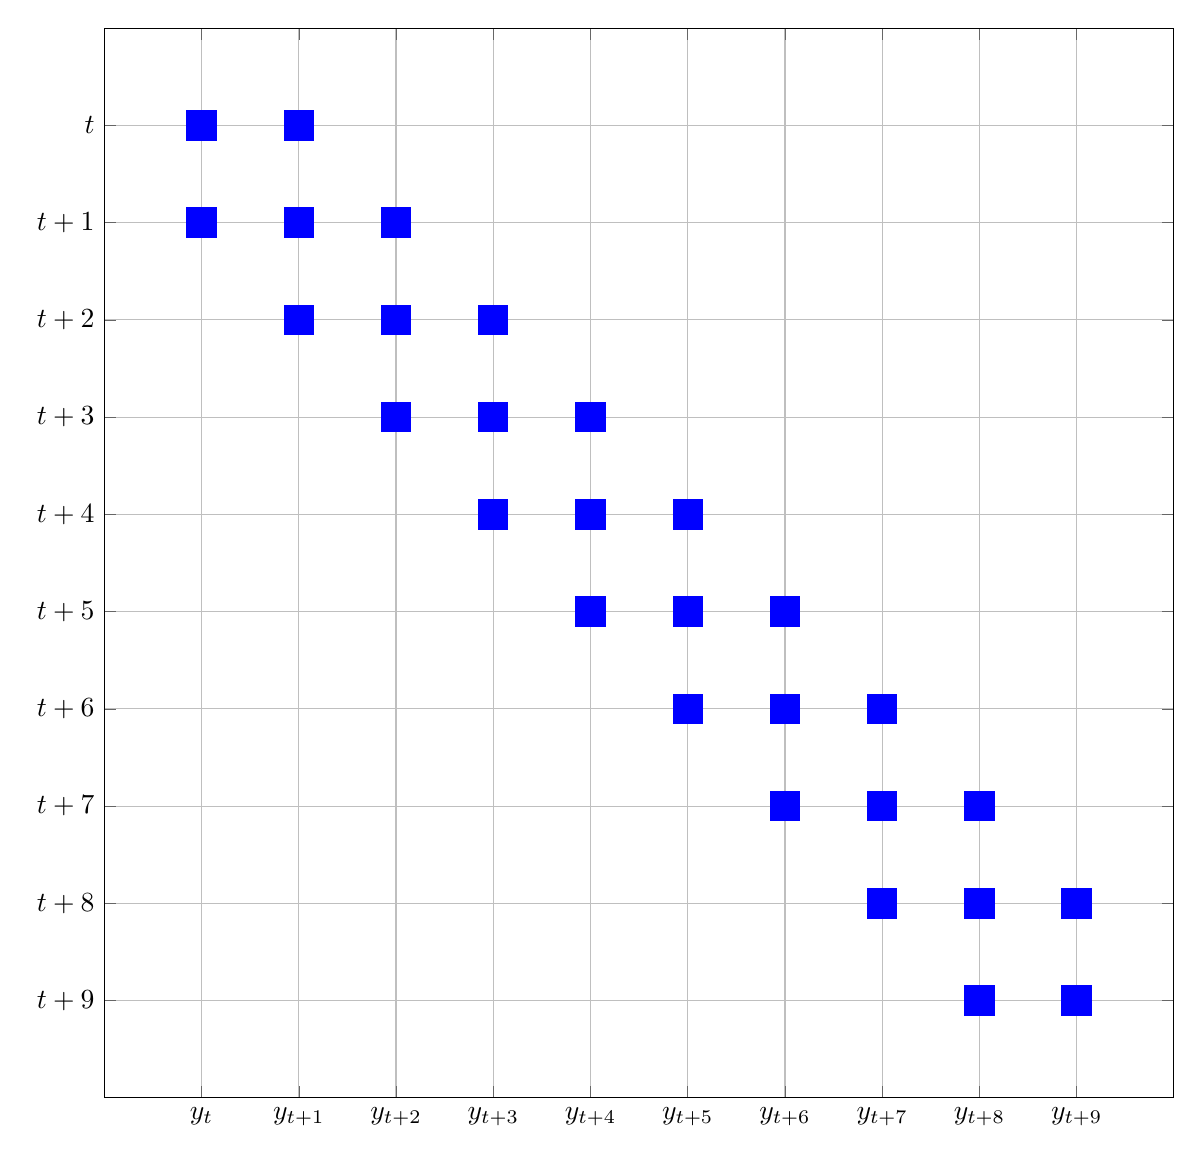
\begin{tikzpicture}

\begin{axis}[%
width=5.348in,
height=5.348in,
at={(1.854in,0.722in)},
scale only axis,
xmin=0,
xmax=11,
xtick={1,2,3,4,5,6,7,8,9,10},
xticklabels={{$y_t$},{$y_{t+1}$},{$y_{t+2}$},{$y_{t+3}$},{$y_{t+4}$},{$y_{t+5}$},{$y_{t+6}$},{$y_{t+7}$},{$y_{t+8}$},{$y_{t+9}$}},
y dir=reverse,
ymin=0,
ymax=11,
ytick={1,2,3,4,5,6,7,8,9,10},
yticklabels={{$t$},{$t+1$},{$t+2$},{$t+3$},{$t+4$},{$t+5$},{$t+6$},{$t+7$},{$t+8$},{$t+9$}},
axis background/.style={fill=white},
xmajorgrids,
ymajorgrids
]
\addplot [color=blue, only marks, mark size=5.3pt, mark=square*, mark options={solid, blue}, forget plot]
  table[row sep=crcr]
  \end{center}
\end{frame}


\begin{frame}
  \frametitle{Extended path}

\begin{itemize}
    \item Unexpected shocks in each period\newline
    \item Loop over perfect foresight models\newline
\end{itemize}

\medskip

\algsetup{
linenosize=\small,
linenodelimiter=.
}
\begin{algorithm}[H]
  \caption{Extended path algorithm}
  \label{alg:ep}
  \begin{algorithmic}[1]
    \STATE $H \leftarrow$ Set the horizon of the perfect foresight (PF) model.
    \STATE $y^\star \leftarrow$ Compute steady state of the model
    \STATE $y_{t-1} \leftarrow$ Choose an initial condition for the state variables
    \FOR{$\tau=t$ to $t+H-1$}
    \STATE $u_\tau  \leftarrow$ Draw random shocks for the current period
    \STATE $y_t \leftarrow$ Solve a PF with $y_{t+H}=y^{\star}$
    \ENDFOR
  \end{algorithmic}
\end{algorithm}

\end{frame}


\begin{frame}
  \frametitle{Approximate expectation}

\begin{itemize}
  \item Use gaussian quadrature
\[
\mathbb E \left[\varphi (X)\right] = \int \varphi(x)f(x)\mathrm dx \approx \sum_{i=1}^m \omega_i \varphi(x_i)
\]
where $(\omega_i,x_i)_{i=1}^m$ are the gaussian quadrature weight and nodes.\newline

\item If more than one source of future uncertainty, use tensor product (default in Dynare).\newline

\item[$\Rightarrow$] First curse of dimensionality.\newline

\item Use unscented transform (Julier et at., 2000): number of nodes grows linearly w.r.t the number of shocks.

\end{itemize}

\end{frame}


\begin{frame}[c]
  \frametitle{Tree of forward histories (second curse)}

\begin{center}
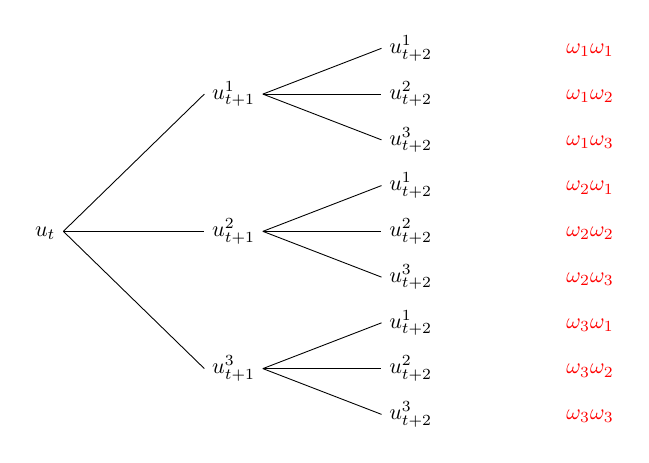
\begin{tikzpicture}[scale=.8]
    \tikzset{grow'=right,level distance=80pt}
    \tikzset{execute at begin node=\strut}
    \tikzset{every tree node/.style={anchor=base west}}
    \Tree [.$u_t$ [.$u^1_{t+1}$ [.$u^1_{t+2}$  \edge[white]; \color{red}{$\omega_1\omega_1$} ]
                          [.$u^2_{t+2}$   \edge[white]; \color{red}{$\omega_1\omega_2$} ]
                          [.$u^3_{t+2}$  \edge[white];
                            \color{red}{$\omega_1\omega_3$} ]]
          [.$u^2_{t+1}$ [.$u^1_{t+2}$  \edge[white]; \color{red}{$\omega_2\omega_1$} ]
                          [.$u^2_{t+2}$   \edge[white]; \color{red}{$\omega_2\omega_2$} ]
                          [.$u^3_{t+2}$  \edge[white];
                            \color{red}{$\omega_2\omega_3$} ]]
          [.$u^3_{t+1}$ [.$u^1_{t+2}$  \edge[white]; \color{red}{$\omega_3\omega_1$} ]
                          [.$u^2_{t+2}$   \edge[white]; \color{red}{$\omega_3\omega_2$} ]
                          [.$u^3_{t+2}$  \edge[white]; \color{red}{$\omega_3\omega_3$} ]]]
  \end{tikzpicture}
\end{center}
\end{frame}





\begin{frame}[c]{}
  \frametitle{Stochastic perfect foresight models}
  \framesubtitle{order 1}
  \centering
  \[
    \begin{split}
      &\sum_{i=1}^m\omega_i f\left( {\color{blue} y_{t-1}}, {\color{red} y_t}, y_{t+1}^i\right) = 0\\
      \begin{sideways}\hspace{-.6cm}\footnotesize{i=1,\dots,m}\end{sideways} &\begin{sqcases}
        f\left( {\color{red}y_t}, y_{t+1}^i, y_{t+2}^i, \epsilon_i \right) = 0\\
        f\left( y_{t+1}^i, y_{t+2}^i, y_{t+3}^i, 0 \right) = 0\\
        \vdots\\
        f\left( y_{t+H-2}^i, y_{t+H-1}^i, {\color{blue}y^{\star}}, 0 \right) = 0\\
      \end{sqcases}
    \end{split}
  \]

\end{frame}


\begin{frame}[c,fragile]{}
  \frametitle{Stochastic perfect foresight models}
  \framesubtitle{order 1}
  \centering

  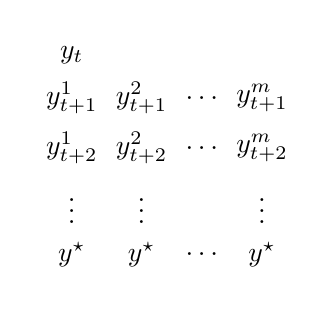
\begin{tikzpicture}
\matrix
  {
    \node {$y_t$}; & \node{}; & \node {}; & \node {}; \\
    \node {$y_{t+1}^1$}; & \node{$y_{t+1}^2$}; & \node{$\ldots$};& \node{$y_{t+1}^m$}; \\
    \node {$y_{t+2}^1$}; & \node{$y_{t+2}^2$}; & \node{$\ldots$};& \node{$y_{t+2}^m$}; \\
    \node {$\vdots$}; & \node{$\vdots$}; & \node{};& \node{$\vdots$}; \\
    \node {$y^\star$}; & \node{$y^\star$}; & \node{$\ldots$};& \node{$y^\star$}; \\
  };
\end{tikzpicture}

\end{frame}



\begin{frame}
  \frametitle{Stochastic perfect foresight model}
  \framesubtitle{Stacked jacobian, order=1, three nodes}
  \begin{center}
    \scalebox{.5}{
  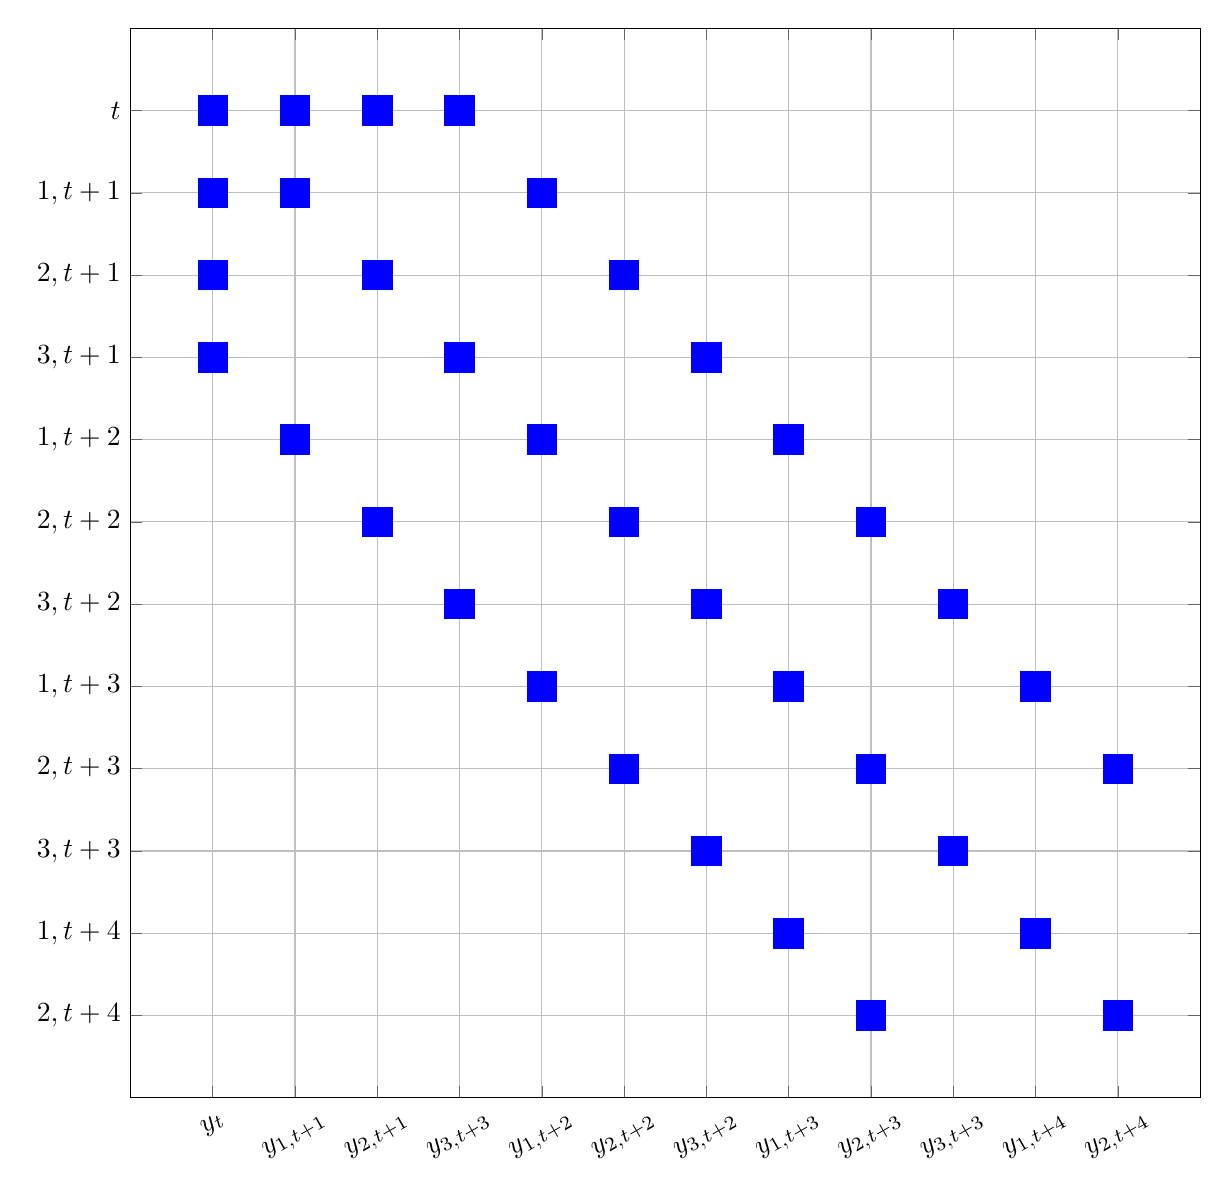
\begin{tikzpicture}

\begin{axis}[%
width=5.348in,
height=5.348in,
at={(1.854in,0.722in)},
scale only axis,
xmin=0,
xmax=13,
xtick={1,2,3,4,5,6,7,8,9,10,11,12},
xticklabels={$y_t$,$y_{1,t+1}$,$y_{2,t+1}$,$y_{3,t+3}$,$y_{1,t+2}$,$y_{2,t+2}$,$y_{3,t+2}$,$y_{1,t+3}$,$y_{2,t+3}$,$y_{3,t+3}$,$y_{1,t+4}$,$y_{2,t+4}$},
xticklabel style={rotate=30},
y dir=reverse,
ymin=0,
ymax=13,
ytick={1,2,3,4,5,6,7,8,9,10,11,12},
yticklabels={$t$,{$1,t+1$},{$2,t+1$},{$3,t+1$},{$1,t+2$},{$2,t+2$},{$3,t+2$},{$1,t+3$},{$2,t+3$},{$3,t+3$},{$1,t+4$},{$2,t+4$}},
axis background/.style={fill=white},
xmajorgrids,
ymajorgrids
]
\addplot [color=blue, only marks, mark size=5.3pt, mark=square*, mark options={solid, blue}, forget plot]
  table[row sep=crcr]
  \end{center}
\end{frame}


  \begin{frame}[c]{}
  \frametitle{Stochastic perfect foresight models}
  \framesubtitle{order 2}
  \centering

  \[
    \begin{split}
      &\sum_{i=1}^m\omega_i f\left( {\color{blue} y_{t-1}}, {\color{red} y_t}, y_{t+1}^i\right) = 0\\
      \begin{sideways}\hspace{-.6cm}\footnotesize{i=1,\dots,m}\end{sideways} & \begin{sqcases}
        \sum_{j=1}^m\omega_jf\left( {\color{red}y_t}, y_{t+1}^j, y_{t+2}^{j,i}, \epsilon_i \right) = 0\\
        \begin{sideways}\hspace{-.6cm}\footnotesize{j=1,\dots,m}\end{sideways} \begin{sqcases}
          f\left( y_{t+1}^i, y_{t+2}^{j,i}, y_{t+3}^{j,i}, \epsilon_j \right) = 0\\
          f\left( y_{t+2}^{j,i}, y_{t+3}^{j,i}, y_{t+4}^{j,i}, 0 \right) = 0\\
          \vdots\\
          f\left(y_{t+H-2}^{j,i} , y_{t+H-1}^{j,i}, {\color{blue}y^{\star}}, 0 \right) = 0
        \end{sqcases}
      \end{sqcases}
    \end{split}
  \]

  \end{frame}


  \begin{frame}[c,fragile]{}
  \frametitle{Stochastic perfect foresight models}
  \framesubtitle{order 2}
  \centering

  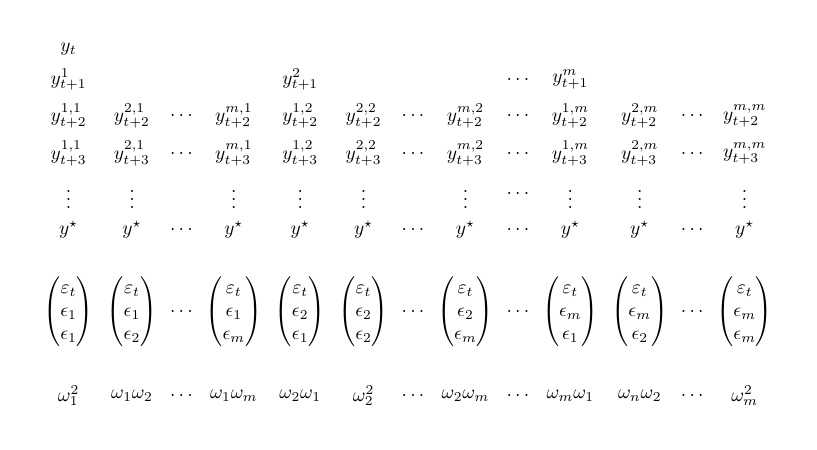
\begin{tikzpicture}[scale=0.7, every node/.style={scale=0.7}]
\matrix
  {
    \node {$y_t$}; & \node{}; & \node {}; & \node {}; \node {}; & \node{}; & \node {}; & \node {}; & \node{}; & \node{}; & \node {}; & \node {}; & \node{};\\
    \node {$y_{t+1}^1$}; & \node{}; & \node{}; & \node{}; & \node {$y_{t+1}^2$}; & \node{}; & \node{}; & \node{}; & \node{$\ldots$}; & \node {$y_{t+1}^m$}; & \node{}; & \node{}; & \node{}; \\
    \node {$y_{t+2}^{1,1}$}; & \node{$y_{t+2}^{2,1}$}; & \node{$\ldots$}; & \node{$y_{t+2}^{m,1}$}; & \node {$y_{t+2}^{1,2}$}; & \node{$y_{t+2}^{2,2}$}; & \node{$\ldots$}; & \node{$y_{t+2}^{m,2}$}; & \node{$\ldots$}; & \node {$y_{t+2}^{1,m}$}; & \node{$y_{t+2}^{2,m}$}; & \node{$\ldots$};& \node{$y_{t+2}^{m,m}$}; \\
    \node {$y_{t+3}^{1,1}$}; & \node{$y_{t+3}^{2,1}$}; & \node{$\ldots$}; & \node{$y_{t+3}^{m,1}$}; & \node {$y_{t+3}^{1,2}$}; & \node{$y_{t+3}^{2,2}$}; & \node{$\ldots$};& \node{$y_{t+3}^{m,2}$}; & \node{$\ldots$}; & \node {$y_{t+3}^{1,m}$}; & \node{$y_{t+3}^{2,m}$}; & \node{$\ldots$};& \node{$y_{t+3}^{m,m}$};\\
    \node {$\vdots$}; & \node{$\vdots$}; & \node{};& \node{$\vdots$}; & \node {$\vdots$}; & \node{$\vdots$}; & \node{};& \node{$\vdots$}; & \node{$\ldots$}; & \node {$\vdots$}; & \node{$\vdots$}; & \node{};& \node{$\vdots$};\\
    \node {$y^\star$}; & \node{$y^\star$}; & \node{$\ldots$};& \node{$y^\star$}; & \node {$y^\star$}; & \node{$y^\star$}; & \node{$\ldots$};& \node{$y^\star$}; & \node{$\ldots$}; & \node {$y^\star$}; & \node{$y^\star$}; & \node{$\ldots$};& \node{$y^\star$};\\
\node {}; & \node{}; & \node{};& \node{}; & \node {}; & \node{}; & \node{};& \node{}; & \node{}; & \node {}; & \node{}; & \node{};& \node{};\\
\node {}; & \node{}; & \node{};& \node{}; & \node {}; & \node{}; & \node{};& \node{}; & \node{}; & \node {}; & \node{}; & \node{};& \node{};\\
\node {$\begin{pmatrix}\varepsilon_t\\ \epsilon_1 \\ \epsilon_1\end{pmatrix}$}; & \node{$\begin{pmatrix}\varepsilon_t\\ \epsilon_1 \\ \epsilon_2\end{pmatrix}$}; & \node{$\ldots$};& \node{$\begin{pmatrix}\varepsilon_t\\ \epsilon_1 \\ \epsilon_m\end{pmatrix}$}; & \node {$\begin{pmatrix}\varepsilon_t\\ \epsilon_2 \\ \epsilon_1\end{pmatrix}$}; & \node{$\begin{pmatrix}\varepsilon_t\\ \epsilon_2 \\ \epsilon_2\end{pmatrix}$}; & \node{$\ldots$};& \node{$\begin{pmatrix}\varepsilon_t\\ \epsilon_2 \\ \epsilon_m\end{pmatrix}$}; & \node{$\ldots$}; & \node {$\begin{pmatrix}\varepsilon_t\\ \epsilon_m \\ \epsilon_1\end{pmatrix}$}; & \node{$\begin{pmatrix}\varepsilon_t\\ \epsilon_m \\ \epsilon_2\end{pmatrix}$}; & \node{$\ldots$};& \node{$\begin{pmatrix}\varepsilon_t\\ \epsilon_m \\ \epsilon_m\end{pmatrix}$};\\
\node {}; & \node{}; & \node{};& \node{}; & \node {}; & \node{}; & \node{};& \node{}; & \node{}; & \node {}; & \node{}; & \node{};& \node{};\\
\node {}; & \node{}; & \node{};& \node{}; & \node {}; & \node{}; & \node{};& \node{}; & \node{}; & \node {}; & \node{}; & \node{};& \node{};\\
\node {$\omega_1^2$}; & \node{$\omega_1\omega_2$}; & \node{$\ldots$};& \node{$\omega_1\omega_m$}; & \node {$\omega_2\omega_1$}; & \node{$\omega_2^2$}; & \node{$\ldots$};& \node{$\omega_2\omega_m$}; & \node{$\ldots$}; & \node {$\omega_m\omega_1$}; & \node{$\omega_n\omega_2$}; & \node{$\ldots$};& \node{$\omega_m^2$};\\
  };
\end{tikzpicture}

\end{frame}


\begin{frame}
    \frametitle{Stochastic perfect foresight model}
    \framesubtitle{Stacked jacobian, order=2, three nodes}
  \begin{center}
    \scalebox{.5}{
  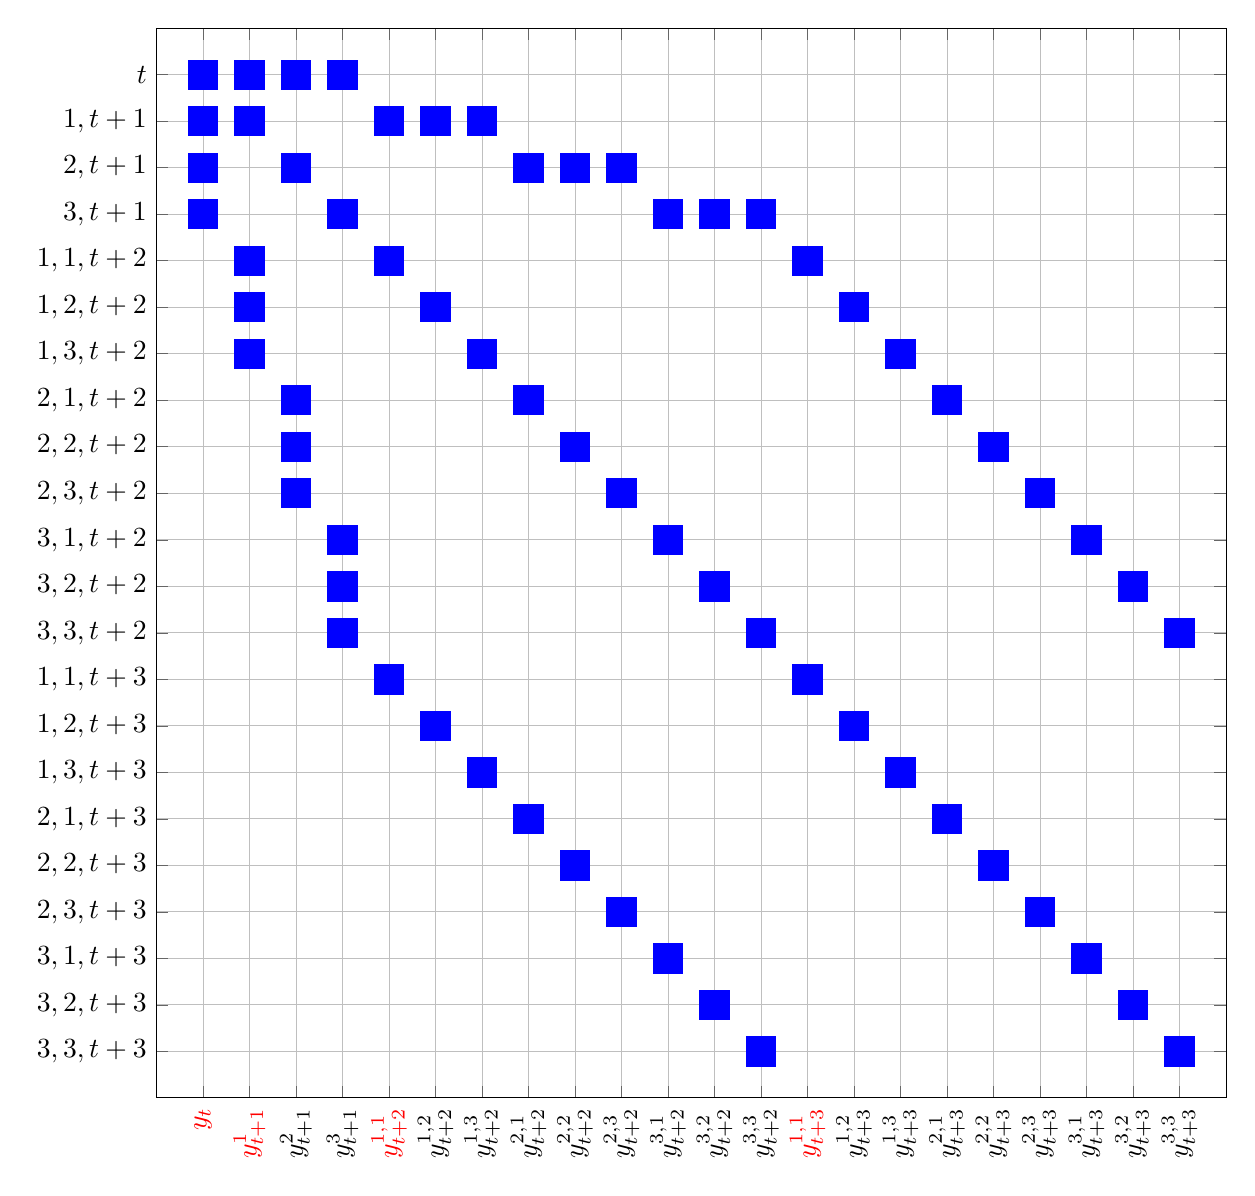
\begin{tikzpicture}

\begin{axis}[%
width=5.348in,
height=5.348in,
at={(1.854in,0.722in)},
scale only axis,
xmin=0,
xmax=23,
xtick={1,2,3,4,5,6,7,8,9,10,11,12,13,14,15,16,17,18,19,20,21,22},
xticklabels={{\color{red}$y_t$},{\color{red}$y_{t+1}^1$},{$y_{t+1}^2$},{$y_{t+1}^3$},{\color{red}$y_{t+2}^{1,1}$},{$y_{t+2}^{1,2}$},{$y_{t+2}^{1,3}$},{$y_{t+2}^{2,1}$},{$y_{t+2}^{2,2}$},{$y_{t+2}^{2,3}$},{$y_{t+2}^{3,1}$},{$y_{t+2}^{3,2}$},{$y_{t+2}^{3,3}$},{\color{red}$y_{t+3}^{1,1}$},{$y_{t+3}^{1,2}$},{$y_{t+3}^{1,3}$},{$y_{t+3}^{2,1}$},{$y_{t+3}^{2,2}$},{$y_{t+3}^{2,3}$},{$y_{t+3}^{3,1}$},{$y_{t+3}^{3,2}$},{$y_{t+3}^{3,3}$}},
xticklabel style={rotate=90},
y dir=reverse,
ymin=0,
ymax=23,
ytick={1,2,3,4,5,6,7,8,9,10,11,12,13,14,15,16,17,18,19,20,21,22},
yticklabels={$t$,{$1,t+1$},{$2,t+1$},{$3,t+1$},{$1,1,t+2$},{$1,2,t+2$},{$1,3,t+2$},{$2,1,t+2$},{$2,2,t+2$},{$2,3,t+2$},{$3,1,t+2$},{$3,2,t+2$},{$3,3,t+2$},{$1,1,t+3$},{$1,2,t+3$},{$1,3,t+3$},{$2,1,t+3$},{$2,2,t+3$},{$2,3,t+3$},{$3,1,t+3$},{$3,2,t+3$},{$3,3,t+3$}},
axis background/.style={fill=white},
xmajorgrids,
ymajorgrids
]
\addplot [color=blue, only marks, mark size=5.3pt, mark=square*, mark options={solid, blue}, forget plot]
  table[row sep=crcr]
  \end{center}

\end{frame}


\begin{frame}
    \frametitle{Stochastic perfect foresight model}
    \framesubtitle{Stacked jacobian, sparse tree, order=2, three nodes}
  \begin{center}
    \scalebox{.6}{
  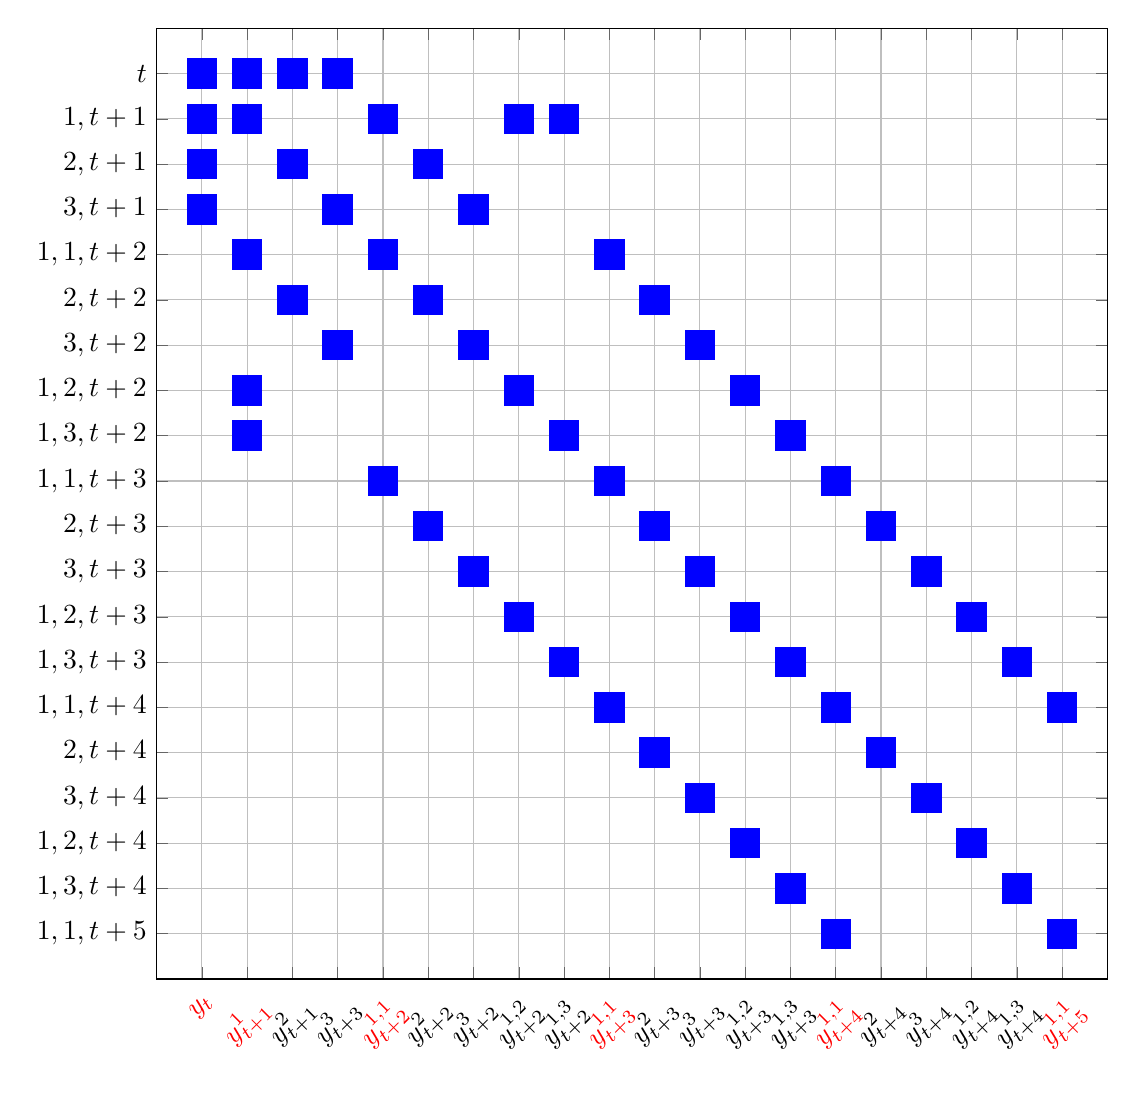
\begin{tikzpicture}

\begin{axis}[%
width=4.754in,
height=4.754in,
at={(1.648in,0.642in)},
scale only axis,
xmin=0,
xmax=21,
xtick={1,2,3,4,5,6,7,8,9,10,11,12,13,14,15,16,17,18,19,20},
xticklabels={{\color{red}$y_{t}$},{\color{red}$y_{t+1}^1$},{$y_{t+1}^2$},{$y_{t+3}^3$},{\color{red}$y_{t+2}^{1,1}$},{$y_{t+2}^2$},{$y_{t+2}^3$},{$y_{t+2}^{1,2}$},{$y_{t+2}^{1,3}$},{\color{red}$y_{t+3}^{1,1}$},{$y_{t+3}^2$},{$y_{t+3}^3$},{$y_{t+3}^{1,2}$},{$y_{t+3}^{1,3}$},{\color{red}$y_{t+4}^{1,1}$},{$y_{t+4}^2$},{$y_{t+4}^3$},{$y_{t+4}^{1,2}$},{$y_{t+4}^{1,3}$},{\color{red}$y_{t+5}^{1,1}$}},
xticklabel style={rotate=45},
y dir=reverse,
ymin=0,
ymax=21,
ytick={1,2,3,4,5,6,7,8,9,10,11,12,13,14,15,16,17,18,19,20},
yticklabels={{$t$},{$1,t+1$},{$2,t+1$},{$3,t+1$},{$1,1,t+2$},{$2,t+2$},{$3,t+2$},{$1,2,t+2$},{$1,3,t+2$},{$1,1,t+3$},{$2,t+3$},{$3,t+3$},{$1,2,t+3$},{$1,3,t+3$},{$1,1,t+4$},{$2,t+4$},{$3,t+4$},{$1,2,t+4$},{$1,3,t+4$},{$1,1,t+5$}},
axis background/.style={fill=white},
xmajorgrids,
ymajorgrids
]
\addplot [color=blue, only marks, mark size=5.3pt, mark=square*, mark options={solid, blue}, forget plot]
  table[row sep=crcr]
  \end{center}

\end{frame}


\begin{frame}
  \frametitle{Burnside (1998) asset pricing model}

\begin{itemize}

  \item The price/dividend ratio and the growth rate of dividends:
  \[
    \begin{split}
      y_t &= \beta \mathbb E_t\left[e^{\theta x_{t+1}}\left(1+y_{t+1}\right)\right]\\
      x_t &= (1-\rho)\bar x + \rho x_{t-1}+\epsilon_t
    \end{split}
  \]

  \item The exact solution is:
\[
    y_t = \sum_{i=1}^\infty \beta^i e^{a_i+b_i\hat x_t}
\]
where
\[
    a_i = \theta \bar x i +
\frac{\theta^2\sigma^2}{2(1-\rho)^2}\left(i-2\rho\frac{1-\rho^i}{1-\rho}+\rho^2\frac{1-\rho^{2i}}{1-\rho^2}\right)
\]
and
\[
b_i = \frac{\theta\rho\left(1-\rho^i\right)}{1-\rho}
\]

\end{itemize}

\end{frame}


\begin{frame}
  \frametitle{Numerical simulation}
   \framesubtitle{Calibration}

\begin{align*}
  \bar x &= 0.0179\\
  \rho &=  -0.139\\
  \theta &= -1.5\\
  \beta &= 0.95\\
  \sigma &= 0.0348\\
\end{align*}

\medskip

\begin{itemize}
\item The deterministic steady state is equal to 12.3035.\newline
\item The risky steady state, defined as the fix point in absence of
  shock this period:
\[
\widetilde y = \sum_{i=1}^\infty \beta^i e^{\theta \bar x i +
\frac{\theta^2\sigma^2}{2(1-\rho)^2}\left(i-2\rho\frac{1-\rho^i}{1-\rho}+\rho^2\frac{1-\rho^{2i}}{1-\rho^2}\right)}\approx 12.4812
\]

\end{itemize}

\end{frame}

\begin{frame}
\frametitle{Comparing SEP, perturbation and closed-form solution}

Simulate long time series ($T=8000$) and compare with true solution. We use a quadrature with 3 nodes for SEP.\newline

\bigskip

\begin{tabular}{l|cc|cc}
  \hline
  & P(1) & P(2) & SEP(0) & SEP(2)\\ \hline
  $100\times\textrm{mean}(|\hat y_t - y_t|/y_t)$  & 1.4261 &  0.0193 & 1.4241 &  1.2534\\
  $100\times\textrm{max}(|\hat y_t - y_t|/y_t)$   & 1.4707 &  0.0527 & 1.4250 &  1.2539\\ \hline\hline
\end{tabular}

\bigskip\bigskip

One can show, using the closed for solution and considering an infinite number of weights and nodes in the quadrature, that we would have to consider an approximation order greater than 60, to be able to recover the theoretical mean of the price-dividend ratio.


\end{frame}



\begin{frame}
  \frametitle{Hybrid approach}

\begin{itemize}

  \item Consider a Taylor expansion of the original problem only along the scale $\sigma$ of the shocks\newline

  \item Use the second order correction for the constant.\newline

  \item[$\Rightarrow$] For K-order SEP, replace $y_{t+K+1}$ in the equations in period $K$ by $y_{t+K+1}+\frac{1}{2}g_{\sigma\sigma}$.\newline

\end{itemize}

\bigskip

\scalebox{.9}{
\begin{tabular}{l|c|ccc}
  \hline
  & P(2) & SEP(2) & SEP(2+) & SEP(10+)\\ \hline
  $100\times\textrm{mean}(|\hat y_t - y_t|/y_t)$  & 0.0193 & 1.2534 & 0.0165 & 0.0153\\
  $100\times\textrm{max}(|\hat y_t - y_t|/y_t)$   & 0.0527 & 1.2539 & 0.0179 & 0.0170\\ \hline\hline
\end{tabular}}

\end{frame}


\begin{frame}
  \frametitle{Irreversible investment}
Consider the following RBC model with irreversible investment:
\[
  \begin{split}
    \max_{\{c_{t+j},l_{t+j},k_{t+j+1}\}_{j=0}^{\infty}} &\quad \mathcal W_t = \sum_{j=0}^{\infty}\beta^ju(c_{t+j},l_{t+j})\\
           \underline{s.t.}   &  \\
              \qquad y_t &= c_t + i_t\\
              \qquad y_t &= A_tf(k_{t},l_t)\\
              \qquad k_{t+1} &= i_t + (1-\delta)k_{t}\\
              \qquad A_{t} &= {A^{\star}}e^{a_{t}}\\
              \qquad a_{t} &= \rho a_{t-1} + \varepsilon_t\\
              \qquad i_t &\ge 0
  \end{split}
\]
\end{frame}

\begin{frame}
\frametitle{Further specifications}
The utility function is
\[
  u(c_t,l_t) = \frac{\left(c_t^{\theta}(1-l_t)^{1-\theta}\right)^{\tau}}{1-\tau}
\]
and the production function,
\[
  f(k_{t},l_t) = \left(\alpha k_{t}^{\psi} + (1-\alpha)l_t^{\psi}\right)^{\frac{1}{\psi}}
\]
\end{frame}

\begin{frame}
\frametitle{First order conditions}
{\footnotesize\[
\begin{split}
  u_c(c_t,l_t) - \mu_t &= \beta \mathbb E_t\Big[
    u_c(c_{t+1},l_{t+1})\Bigl(A_{t+1}f_k(k_{t+1},l_{t+1}) + 1
    -\delta\Bigr) - \mu_{t+1}(1-\delta)\Big]\\
  \frac{u_{l}(c_t,l_t)}{u_c(c_t,l_t)} &= A_tf_l(k_t,l_t)\\
  c_t + k_{t+1} &= A_tf(k_{t},l_t) + (1-\delta)k_{t}\\
  0 &= \mu_t \left( k_{t+1} - (1-\delta)k_{t} \right)
\end{split}
\]}

\bigskip\bigskip

where $\mu_t$ is the Lagrange multiplier associated with the constraint on investment.
\end{frame}

\begin{frame}
  \frametitle{Calibration}
  \begin{align*}
    \beta    &=  0.990\\
    \theta   &=  0.357\\
    \tau     &=  2.000\\
    \alpha   &=  0.450\\
    \psi     &= -0.500\\
    \delta   &=  0.010\\
    \rho     &=  0.800\\
    A^\star &=  1.000\\
    \sigma   &=  0.100
  \end{align*}
\end{frame}


\begin{frame}
    \frametitle{Simulation of the RBC model}
    \framesubtitle{SEP with orders=0,\dots,10}
  \begin{center}
    \scalebox{.5}{
  % This file was created by matlab2tikz.
%
%The latest updates can be retrieved from
%  http://www.mathworks.com/matlabcentral/fileexchange/22022-matlab2tikz-matlab2tikz
%where you can also make suggestions and rate matlab2tikz.
%
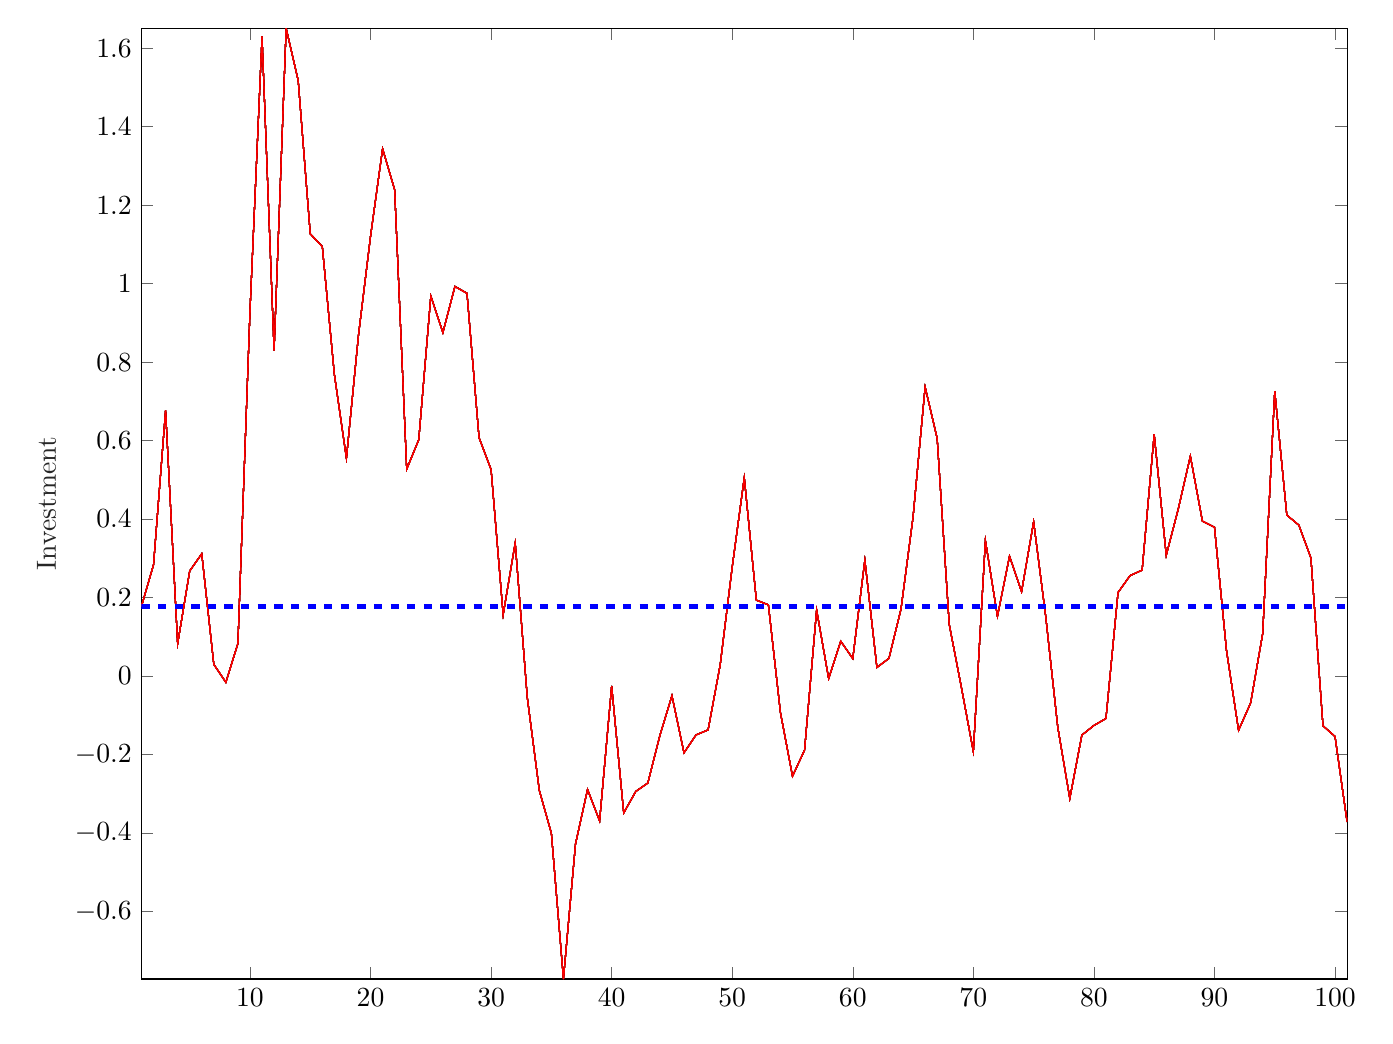
\begin{tikzpicture}

\begin{axis}[%
width=6.028in,
height=4.754in,
at={(1.011in,0.642in)},
scale only axis,
xmin=1,
xmax=101,
ymin=-0.772195006292555,
ymax=1.65088357931635,
ylabel style={font=\color{white!15!black}},
ylabel={Investment},
axis background/.style={fill=white}
]
\addplot [color=black, forget plot]
  table[row sep=crcr]{%
1	0.177702040741409\\
2	0.283678871039512\\
3	0.677124839755998\\
4	0.0824838016040461\\
5	0.267863391883711\\
6	0.311717571374166\\
7	0.0299523950325572\\
8	-0.015725759818706\\
9	0.0832350956043053\\
10	0.929403649185558\\
11	1.62986695278717\\
12	0.829309708082963\\
13	1.65088357931635\\
14	1.51773699481356\\
15	1.12710990490289\\
16	1.09470509002036\\
17	0.76884906834339\\
18	0.555385346426014\\
19	0.868947240413062\\
20	1.1211005312356\\
21	1.34413428881577\\
22	1.23963275687048\\
23	0.527635342381533\\
24	0.602658485501459\\
25	0.968755548588763\\
26	0.875690999351196\\
27	0.993273647230984\\
28	0.975802803657734\\
29	0.607895596454024\\
30	0.526533842556063\\
31	0.156692748648537\\
32	0.339884246926733\\
33	-0.0539016910897512\\
34	-0.291183556431799\\
35	-0.400342222857124\\
36	-0.771753968678462\\
37	-0.427860590450035\\
38	-0.288819685173126\\
39	-0.368873043272291\\
40	-0.0251893339851563\\
41	-0.348627708816666\\
42	-0.293900324183\\
43	-0.272473930519342\\
44	-0.151336923981497\\
45	-0.0499391622283405\\
46	-0.195438439604022\\
47	-0.149900754743346\\
48	-0.137109993578672\\
49	0.0282365061130416\\
50	0.278059838075542\\
51	0.505772946870918\\
52	0.193564365730037\\
53	0.181593734282649\\
54	-0.0930779308524574\\
55	-0.255262920409647\\
56	-0.188685256158933\\
57	0.168484045020259\\
58	-0.00637627390945669\\
59	0.0888555295256739\\
60	0.0445221354652522\\
61	0.295674761249941\\
62	0.0220973609060398\\
63	0.0451173623301888\\
64	0.170828191695543\\
65	0.405317539123377\\
66	0.736837253638714\\
67	0.60561814524846\\
68	0.131603728070542\\
69	-0.0274427336119486\\
70	-0.192454758864625\\
71	0.345298503468049\\
72	0.152349668273311\\
73	0.305545475705741\\
74	0.215044646508763\\
75	0.393091169537991\\
76	0.152618360465428\\
77	-0.129666789779723\\
78	-0.311903255143949\\
79	-0.150632756753248\\
80	-0.125920045604308\\
81	-0.108215366215278\\
82	0.212828607558224\\
83	0.255962831129138\\
84	0.269921891164909\\
85	0.616183704012109\\
86	0.307901017443085\\
87	0.426026400168025\\
88	0.560369498334127\\
89	0.394868527978671\\
90	0.379290893982795\\
91	0.0647415367362655\\
92	-0.138322687553493\\
93	-0.0684456440312256\\
94	0.108063251687653\\
95	0.726216540339419\\
96	0.410285036702756\\
97	0.384673652038146\\
98	0.300894665523511\\
99	-0.126787267598739\\
100	-0.153951324691751\\
101	-0.371786880503128\\
};
\addplot [color=black!90!red, forget plot]
  table[row sep=crcr]{%
1	0.177702040741409\\
2	0.283577070429264\\
3	0.677068866261966\\
4	0.0823531930551838\\
5	0.267757050802386\\
6	0.311616480466258\\
7	0.0298217125539751\\
8	-0.0158562778663827\\
9	0.0831200480878623\\
10	0.929378619634449\\
11	1.62989478605484\\
12	0.829234000293024\\
13	1.65086790820188\\
14	1.51768144580654\\
15	1.12700172514281\\
16	1.09458088214932\\
17	0.768692244690184\\
18	0.555210945955072\\
19	0.868788289503828\\
20	1.12094791850825\\
21	1.3439815895878\\
22	1.23946070001786\\
23	0.527424187833049\\
24	0.602449989579328\\
25	0.968558089126593\\
26	0.875484350327405\\
27	0.993065608787104\\
28	0.975588182280527\\
29	0.607667996498382\\
30	0.526304745786758\\
31	0.156460389474167\\
32	0.339658685016799\\
33	-0.0541265422371268\\
34	-0.291401146760158\\
35	-0.400550077373086\\
36	-0.771946387530972\\
37	-0.428045180953002\\
38	-0.288994702612987\\
39	-0.369039489788191\\
40	-0.0253459112919452\\
41	-0.348779547273684\\
42	-0.294043532057005\\
43	-0.272609129112826\\
44	-0.15146402994995\\
45	-0.050059484451507\\
46	-0.195554666019784\\
47	-0.150010273167126\\
48	-0.137213601984485\\
49	0.0281397130276297\\
50	0.277968779012264\\
51	0.505684250880114\\
52	0.19346987705317\\
53	0.181500462513358\\
54	-0.0931715648472365\\
55	-0.255352582684153\\
56	-0.188767963933157\\
57	0.168409873070412\\
58	-0.00645082147854858\\
59	0.0887851356796231\\
60	0.0444533724532035\\
61	0.295610901542471\\
62	0.0220300967258876\\
63	0.0450531112329557\\
64	0.17076758754364\\
65	0.405259973083657\\
66	0.736780384389107\\
67	0.605552685343264\\
68	0.131529165120157\\
69	-0.0275168827423955\\
70	-0.192526475508228\\
71	0.345236841672261\\
72	0.152284683342731\\
73	0.305482874584346\\
74	0.214980191082026\\
75	0.393028452770243\\
76	0.152551384059885\\
77	-0.12973480230073\\
78	-0.311967910962976\\
79	-0.150689272608266\\
80	-0.125971598096433\\
81	-0.108262431575561\\
82	0.212789397538922\\
83	0.255923659023438\\
84	0.269881801758991\\
85	0.616146597178698\\
86	0.307853911630215\\
87	0.425979136697647\\
88	0.560320582945593\\
89	0.39481260731342\\
90	0.379232272388101\\
91	0.0646773389518748\\
92	-0.138386786506959\\
93	-0.0685042472181875\\
94	0.108010510124984\\
95	0.726172720345419\\
96	0.410229807819033\\
97	0.384615362411725\\
98	0.30083313182062\\
99	-0.126854302000931\\
100	-0.154013978606668\\
101	-0.371847010462909\\
};
\addplot [color=black!80!red, forget plot]
  table[row sep=crcr]{%
1	0.177702040741409\\
2	0.283508883696199\\
3	0.677018091639968\\
4	0.0822721738183649\\
5	0.267686575113668\\
6	0.311548157007619\\
7	0.0297419858135168\\
8	-0.0159347741014776\\
9	0.083048960342534\\
10	0.929339502818691\\
11	1.62986587255508\\
12	0.829167693483451\\
13	1.65081384208249\\
14	1.51760842495678\\
15	1.12690857869407\\
16	1.09447919304528\\
17	0.768579121871078\\
18	0.555092127407932\\
19	0.868671632027758\\
20	1.12082909525352\\
21	1.34385743484279\\
22	1.23932781036823\\
23	0.527283593141482\\
24	0.60230951511313\\
25	0.96841652442651\\
26	0.875339343835899\\
27	0.992917332294075\\
28	0.975436414576655\\
29	0.607515886227017\\
30	0.526153327995636\\
31	0.156313605533946\\
32	0.339512956177126\\
33	-0.0542650434862104\\
34	-0.291531386440332\\
35	-0.400672448116278\\
36	-0.772054018690978\\
37	-0.42815187556769\\
38	-0.289097230492695\\
39	-0.369135196291698\\
40	-0.0254409765163209\\
41	-0.34886616066629\\
42	-0.294125309489847\\
43	-0.272685999788332\\
44	-0.15153778013282\\
45	-0.0501307657421058\\
46	-0.195620605804678\\
47	-0.150072711317741\\
48	-0.137272475369222\\
49	0.0280819177589156\\
50	0.277909107661495\\
51	0.505620579016314\\
52	0.193409944862218\\
53	0.181441574754679\\
54	-0.093224979602416\\
55	-0.255400354071911\\
56	-0.188812441332462\\
57	0.168363346132065\\
58	-0.00649373589534646\\
59	0.0887427857320743\\
60	0.0444130379883115\\
61	0.295567822984792\\
62	0.0219911892051256\\
63	0.0450156154809207\\
64	0.170729525192264\\
65	0.405218047040851\\
66	0.736730059002291\\
67	0.605500713010857\\
68	0.131483143555494\\
69	-0.0275591959788009\\
70	-0.192563885235827\\
71	0.34519388178749\\
72	0.152244247429462\\
73	0.305440289472609\\
74	0.214938606125493\\
75	0.392983612106825\\
76	0.15250963970331\\
77	-0.129771123283642\\
78	-0.311998548928411\\
79	-0.150717690269346\\
80	-0.125997306589145\\
81	-0.108285599063819\\
82	0.212763782729823\\
83	0.255896970189657\\
84	0.269854172827449\\
85	0.616111505513861\\
86	0.307820920558746\\
87	0.425942987330829\\
88	0.560279832015083\\
89	0.394771898167214\\
90	0.379190276338609\\
91	0.0646393421650773\\
92	-0.138420382579914\\
93	-0.0685357364600943\\
94	0.107978811853814\\
95	0.726130441373703\\
96	0.410189122312992\\
97	0.384573426934089\\
98	0.300791257688277\\
99	-0.126890028903955\\
100	-0.154046317632118\\
101	-0.371873557323757\\
};
\addplot [color=black!70!red, forget plot]
  table[row sep=crcr]{%
1	0.177702040741409\\
2	0.283463716096716\\
3	0.67697843683708\\
4	0.0822216395105792\\
5	0.267640251406544\\
6	0.311502616151347\\
7	0.0296929828786143\\
8	-0.0159823920513332\\
9	0.0830047603273759\\
10	0.929303688825187\\
11	1.62982680384185\\
12	0.829116815230739\\
13	1.65075982038627\\
14	1.51754496120137\\
15	1.12683790515062\\
16	1.0944037929511\\
17	0.768500556179763\\
18	0.555012452549209\\
19	0.868589829167975\\
20	1.1207431928853\\
21	1.34376588590859\\
22	1.23923221388592\\
23	0.527190738952696\\
24	0.602215993083724\\
25	0.968318643931697\\
26	0.875240341484908\\
27	0.992815174739154\\
28	0.975332333958432\\
29	0.607415163088389\\
30	0.526053774388324\\
31	0.156220296366418\\
32	0.339418717849917\\
33	-0.0543511619745233\\
34	-0.291610319439204\\
35	-0.400745471431059\\
36	-0.772114799445743\\
37	-0.42821442276156\\
38	-0.289158183101958\\
39	-0.369191028658467\\
40	-0.0254994533462727\\
41	-0.348916194529927\\
42	-0.294172692507635\\
43	-0.272730431506906\\
44	-0.151581311051416\\
45	-0.0501737177403824\\
46	-0.195658595329793\\
47	-0.150108878098267\\
48	-0.137306474806296\\
49	0.0280469168149752\\
50	0.277870074378816\\
51	0.505576369546679\\
52	0.193371682718511\\
53	0.181404063999884\\
54	-0.0932559550121454\\
55	-0.255426016492138\\
56	-0.18883663151363\\
57	0.168333908989595\\
58	-0.00651887977022782\\
59	0.0887169222617407\\
60	0.0443889685970509\\
61	0.295539039718259\\
62	0.0219682844355486\\
63	0.0449933492080429\\
64	0.170705416553033\\
65	0.405188618236567\\
66	0.73669115148559\\
67	0.605462511995441\\
68	0.131454436904971\\
69	-0.0275837448477073\\
70	-0.192583484077175\\
71	0.34516455940585\\
72	0.152218845543616\\
73	0.305411687398052\\
74	0.214911727162815\\
75	0.392952512738237\\
76	0.152483394547738\\
77	-0.129790704010778\\
78	-0.312012508374277\\
79	-0.150731910520148\\
80	-0.126010047134243\\
81	-0.108296896236182\\
82	0.212747029074187\\
83	0.255878986350766\\
84	0.269835415547633\\
85	0.616083519552661\\
86	0.307798307438345\\
87	0.425916878721586\\
88	0.560249111993263\\
89	0.394743345461809\\
90	0.379161114860933\\
91	0.0646165167711244\\
92	-0.138438071513322\\
93	-0.0685528490886093\\
94	0.107959493959728\\
95	0.726096550445539\\
96	0.410160385557055\\
97	0.384544232918889\\
98	0.300763143652291\\
99	-0.126909227443896\\
100	-0.154063018661711\\
101	-0.371884170518498\\
};
\addplot [color=black!60!red, forget plot]
  table[row sep=crcr]{%
1	0.177702040741409\\
2	0.283434037152432\\
3	0.676949586334448\\
4	0.0821899722642245\\
5	0.267609989486647\\
6	0.311472561079978\\
7	0.0296626630456761\\
8	-0.0160115127061854\\
9	0.0829771314131275\\
10	0.929275643069728\\
11	1.62979245350009\\
12	0.829080196408805\\
13	1.65071639225708\\
14	1.51749663374323\\
15	1.12678743154176\\
16	1.09435062187303\\
17	0.768447252716063\\
18	0.554959628292221\\
19	0.868533992070868\\
20	1.12068349553265\\
21	1.34370157821827\\
22	1.23916598917051\\
23	0.527129782472445\\
24	0.602154271845607\\
25	0.968252418313516\\
26	0.875173886467666\\
27	0.99274620850186\\
28	0.975262272393516\\
29	0.607348913967077\\
30	0.525988647087405\\
31	0.15616075713457\\
32	0.339357787141081\\
33	-0.0544055484627307\\
34	-0.291658916436153\\
35	-0.400789477482046\\
36	-0.772149390270324\\
37	-0.42825150293318\\
38	-0.289194829923857\\
39	-0.36922398067487\\
40	-0.0255357316319116\\
41	-0.348945459234741\\
42	-0.29420048477456\\
43	-0.272756384773954\\
44	-0.151607289121529\\
45	-0.0501998418023514\\
46	-0.195680821806294\\
47	-0.150130161581553\\
48	-0.137326359622748\\
49	0.0280253787249397\\
50	0.277844630940624\\
51	0.50554633035824\\
52	0.193347219230373\\
53	0.181380163796405\\
54	-0.093274119302957\\
55	-0.255439895471301\\
56	-0.188849915466598\\
57	0.168315190117058\\
58	-0.00653381339621097\\
59	0.0887009680148426\\
60	0.0443744238094034\\
61	0.295519983130398\\
62	0.0219546176767165\\
63	0.0449799540703929\\
64	0.170690084597407\\
65	0.405168468904046\\
66	0.73666298697932\\
67	0.60543562385233\\
68	0.131436393636073\\
69	-0.0275981802290723\\
70	-0.192593780872382\\
71	0.345144853035415\\
72	0.152202802320795\\
73	0.305392680283788\\
74	0.214894365411095\\
75	0.392931393325157\\
76	0.152466812182759\\
77	-0.129801351119333\\
78	-0.312018465005218\\
79	-0.150738967046962\\
80	-0.126016294459939\\
81	-0.108302319115372\\
82	0.212736094694533\\
83	0.255866993953075\\
84	0.26982284383029\\
85	0.616062889646426\\
86	0.307783059565478\\
87	0.42589867311049\\
88	0.560227155455954\\
89	0.394723807853945\\
90	0.379141292942037\\
91	0.0646026481724168\\
92	-0.138447428547625\\
93	-0.0685622499884619\\
94	0.107947598331768\\
95	0.726071535818964\\
96	0.410140633425171\\
97	0.384524357482496\\
98	0.300744469787128\\
99	-0.126919626950899\\
100	-0.15407164361233\\
101	-0.371887568645549\\
};
\addplot [color=black!50!red, forget plot]
  table[row sep=crcr]{%
1	0.177702040741409\\
2	0.283414652099377\\
3	0.676929422678068\\
4	0.0821700498889678\\
5	0.267590312222802\\
6	0.311452870269701\\
7	0.0296437933861369\\
8	-0.0160294531553401\\
9	0.0829597830362234\\
10	0.929255222250675\\
11	1.62976610989932\\
12	0.82905478744713\\
13	1.65068445104024\\
14	1.51746205769895\\
15	1.12675259402016\\
16	1.09431420492022\\
17	0.768411610361085\\
18	0.554924937382037\\
19	0.868496530879456\\
20	1.12064297973724\\
21	1.34365764599642\\
22	1.23912113193534\\
23	0.527089975768943\\
24	0.602113796297843\\
25	0.968208233602185\\
26	0.875129782480125\\
27	0.992700258635445\\
28	0.9752156803459\\
29	0.607305560676803\\
30	0.525946188729596\\
31	0.156122683194763\\
32	0.339318419677031\\
33	-0.054439693600996\\
34	-0.291688860686866\\
35	-0.400816502818311\\
36	-0.772169233964395\\
37	-0.428273706201273\\
38	-0.28921707559263\\
39	-0.369243635198967\\
40	-0.0255583860655917\\
41	-0.348962764397841\\
42	-0.294216968601249\\
43	-0.272771728022371\\
44	-0.151622967701886\\
45	-0.0502158876129556\\
46	-0.195693932702147\\
47	-0.150142786384432\\
48	-0.137338185664469\\
49	0.0280120987625719\\
50	0.277828097013345\\
51	0.505526220640587\\
52	0.19333155470101\\
53	0.181364893349068\\
54	-0.0932849858073308\\
55	-0.255447456824136\\
56	-0.188857283893585\\
57	0.16830327055186\\
58	-0.00654278699537888\\
59	0.0886910458975782\\
60	0.044365544046972\\
61	0.295507448329062\\
62	0.0219463694551982\\
63	0.0449718087722759\\
64	0.170680311603828\\
65	0.405154906954175\\
66	0.736643353285589\\
67	0.605417200484508\\
68	0.131425020299077\\
69	-0.0276067707256318\\
70	-0.192599208417674\\
71	0.345131760225552\\
72	0.152192631502549\\
73	0.305380154557899\\
74	0.214883161777733\\
75	0.392917259623256\\
76	0.152456306660667\\
77	-0.129807194597335\\
78	-0.312020714939856\\
79	-0.150742429828475\\
80	-0.126019313954845\\
81	-0.108304864807895\\
82	0.212728977736601\\
83	0.255859064385346\\
84	0.269814501852733\\
85	0.616048339586383\\
86	0.307772902003552\\
87	0.425886267125747\\
88	0.56021196045055\\
89	0.394710663488942\\
90	0.379128019404383\\
91	0.0645941431888727\\
92	-0.138452403956106\\
93	-0.0685674731955592\\
94	0.107940215194194\\
95	0.726053891130304\\
96	0.410127304010774\\
97	0.384511029430984\\
98	0.300732169044321\\
99	-0.126925309524022\\
100	-0.154076097170548\\
101	-0.371887949669848\\
};
\addplot [color=black!40!red, forget plot]
  table[row sep=crcr]{%
1	0.177702040741409\\
2	0.283402047718417\\
3	0.676915680392963\\
4	0.0821574751897958\\
5	0.267577562970968\\
6	0.311440039934106\\
7	0.0296319905154316\\
8	-0.0160405785729403\\
9	0.0829488488219922\\
10	0.929240948252421\\
11	1.62974717497514\\
12	0.829037558141629\\
13	1.65066202472589\\
14	1.51743816995571\\
15	1.12672905493353\\
16	1.09428972162179\\
17	0.768388054933811\\
18	0.554902168892357\\
19	0.868471692815282\\
20	1.12061590161153\\
21	1.34362815432339\\
22	1.23909118652365\\
23	0.527064078910855\\
24	0.602087383466347\\
25	0.968179036863522\\
26	0.875100745653608\\
27	0.992669920218352\\
28	0.975184956164048\\
29	0.607277303102138\\
30	0.525918592293694\\
31	0.156098307067792\\
32	0.339293008758769\\
33	-0.0544613038606906\\
34	-0.291707480512974\\
35	-0.400832734582198\\
36	-0.772180710590271\\
37	-0.428287170073495\\
38	-0.289230684902387\\
39	-0.36925546666085\\
40	-0.0255725999049201\\
41	-0.348973098250461\\
42	-0.294226842047917\\
43	-0.272780890884646\\
44	-0.151632515212083\\
45	-0.0502258079808278\\
46	-0.195701759158427\\
47	-0.150150365434856\\
48	-0.137345246101099\\
49	0.0280038366998645\\
50	0.27781738470374\\
51	0.505512902330437\\
52	0.193321522106454\\
53	0.181355129958684\\
54	-0.0932914908547692\\
55	-0.255451610113582\\
56	-0.188861418582959\\
57	0.168295666646565\\
58	-0.00654824528468869\\
59	0.0886848439374216\\
60	0.0443600740532022\\
61	0.295499257913342\\
62	0.0219413434001577\\
63	0.0449668118348064\\
64	0.170674076173502\\
65	0.405145889934454\\
66	0.736629988619842\\
67	0.605404801157906\\
68	0.131417823200597\\
69	-0.0276119502652087\\
70	-0.192602079870303\\
71	0.345123136093813\\
72	0.152186171492202\\
73	0.30537195343571\\
74	0.2148759453416\\
75	0.39290790184148\\
76	0.152449616879093\\
77	-0.129810432947682\\
78	-0.312021337847777\\
79	-0.150744102863771\\
80	-0.126020743531897\\
81	-0.108306020328074\\
82	0.212724359026478\\
83	0.255853857605259\\
84	0.269809010474484\\
85	0.616038356449567\\
86	0.30776619781828\\
87	0.42587794712121\\
88	0.560201664355059\\
89	0.394701928214125\\
90	0.379119227506542\\
91	0.0645888886926915\\
92	-0.138455064978539\\
93	-0.0685704089722586\\
94	0.107935605369775\\
95	0.726041788224546\\
96	0.410118426800014\\
97	0.384502195503311\\
98	0.30072411887647\\
99	-0.126928443902538\\
100	-0.154078396382397\\
101	-0.371887251957873\\
};
\addplot [color=black!30!red, forget plot]
  table[row sep=crcr]{%
1	0.177702040741409\\
2	0.283393880469028\\
3	0.676906470722907\\
4	0.0821495165978721\\
5	0.267569325632168\\
6	0.311431714447065\\
7	0.0296245761525122\\
8	-0.0160475176072839\\
9	0.0829419357388435\\
10	0.929231221335995\\
11	1.62973405356358\\
12	0.829026054380381\\
13	1.65064670890485\\
14	1.51742202031097\\
15	1.12671337377469\\
16	1.09427346650303\\
17	0.768372600121405\\
18	0.554887395426479\\
19	0.868455360183418\\
20	1.12059799278437\\
21	1.34360858660043\\
22	1.23907139252357\\
23	0.527047282025067\\
24	0.602070211145541\\
25	0.968159875184741\\
26	0.875081738552049\\
27	0.992650017905315\\
28	0.975164817494014\\
29	0.607258940949569\\
30	0.525900698124152\\
31	0.156082689044027\\
32	0.339276621081919\\
33	-0.0544750181691984\\
34	-0.291719118516634\\
35	-0.400843192448458\\
36	-0.772187384903339\\
37	-0.428295341757475\\
38	-0.289239048261403\\
39	-0.369262631659917\\
40	-0.0255815358619163\\
41	-0.348979310115681\\
42	-0.294232795000286\\
43	-0.272786400017167\\
44	-0.151638361318462\\
45	-0.0502319461895402\\
46	-0.195706464062372\\
47	-0.15015494571121\\
48	-0.137349502376133\\
49	0.0279986800089746\\
50	0.277810469884046\\
51	0.505504158068072\\
52	0.193315106306327\\
53	0.181348893874356\\
54	-0.0932954265135334\\
55	-0.255453901677597\\
56	-0.188863750954224\\
57	0.168290819669212\\
58	-0.00655157321177255\\
59	0.0886809565515299\\
60	0.0443566925202445\\
61	0.295493935105424\\
62	0.0219382608898889\\
63	0.0449637292671843\\
64	0.17067009566266\\
65	0.405139953707796\\
66	0.736621039711212\\
67	0.605396564117056\\
68	0.131413264672729\\
69	-0.0276150828104291\\
70	-0.192603599877701\\
71	0.345117497017388\\
72	0.152182066351325\\
73	0.305366615339682\\
74	0.21487130715316\\
75	0.392901758982753\\
76	0.152445372172921\\
77	-0.129812242053546\\
78	-0.31202130673381\\
79	-0.150744889961921\\
80	-0.126021396619709\\
81	-0.108306513961675\\
82	0.212721372539685\\
83	0.255850460421328\\
84	0.269805420788068\\
85	0.616031633841576\\
86	0.307761808275641\\
87	0.425872433232318\\
88	0.560194790651876\\
89	0.394696177163453\\
90	0.379113453350387\\
91	0.0645856242082867\\
92	-0.138456495198587\\
93	-0.0685720762315549\\
94	0.107932716003411\\
95	0.726033640181365\\
96	0.410112572762029\\
97	0.384496389894916\\
98	0.300718879111845\\
99	-0.126930188104636\\
100	-0.154079581199844\\
101	-0.371886312240348\\
};
\addplot [color=black!20!red, forget plot]
  table[row sep=crcr]{%
1	0.177702040741409\\
2	0.283388602466119\\
3	0.676900370796535\\
4	0.0821444680914521\\
5	0.267564014631647\\
6	0.311426329309996\\
7	0.0296199018446834\\
8	-0.016051866946327\\
9	0.0829375536538364\\
10	0.929224704251713\\
11	1.6297251654956\\
12	0.829018456280639\\
13	1.65063643203749\\
14	1.51741125799351\\
15	1.12670303031718\\
16	1.09426276950266\\
17	0.768362517833441\\
18	0.554877819472452\\
19	0.868444686384834\\
20	1.12058623720483\\
21	1.34359571015925\\
22	1.23905840134316\\
23	0.527036414930936\\
24	0.60205908007773\\
25	0.968147363604678\\
26	0.8750693514276\\
27	0.992637024324723\\
28	0.975151675907492\\
29	0.607247039091898\\
30	0.525889118897199\\
31	0.156072679809965\\
32	0.339266062821828\\
33	-0.0544837377192905\\
34	-0.291726421812951\\
35	-0.400849523247751\\
36	-0.772191305709564\\
37	-0.428300354275157\\
38	-0.289244218075278\\
39	-0.369267006243094\\
40	-0.0255871720806321\\
41	-0.34898307898969\\
42	-0.294236417260369\\
43	-0.272789744181147\\
44	-0.151641968368924\\
45	-0.0502358366909024\\
46	-0.19570931910854\\
47	-0.150157738685018\\
48	-0.137352092155633\\
49	0.027995445896306\\
50	0.277806013443225\\
51	0.50549844900693\\
52	0.19331100491744\\
53	0.181344908348676\\
54	-0.0932978289264775\\
55	-0.25545517941242\\
56	-0.188865083600247\\
57	0.168287726937478\\
58	-0.00655362237931892\\
59	0.0886785097585601\\
60	0.0443545877167715\\
61	0.29549048711085\\
62	0.0219363572648537\\
63	0.0449618283964285\\
64	0.170667556556973\\
65	0.405136070523726\\
66	0.736615113777302\\
67	0.605391140263154\\
68	0.131410371129057\\
69	-0.0276169982922663\\
70	-0.192604409505477\\
71	0.345113827198964\\
72	0.152179453683689\\
73	0.305363153490287\\
74	0.214868328566985\\
75	0.392897749677479\\
76	0.152442670662908\\
77	-0.12981326463287\\
78	-0.312021065194834\\
79	-0.15074524890167\\
80	-0.12602168145447\\
81	-0.108306705345126\\
82	0.212719444870392\\
83	0.255848252714244\\
84	0.269803084768757\\
85	0.616027164281097\\
86	0.307758945425119\\
87	0.425868809126969\\
88	0.560190248893904\\
89	0.394692415735848\\
90	0.379109683772827\\
91	0.0645835977210387\\
92	-0.138457270679601\\
93	-0.068573035330833\\
94	0.107930897501718\\
95	0.726028224389859\\
96	0.410108739247619\\
97	0.384492597820604\\
98	0.300715481570099\\
99	-0.126931169863726\\
100	-0.154080192407155\\
101	-0.37188545626642\\
};
\addplot [color=black!10!red, forget plot]
  table[row sep=crcr]{%
1	0.177702040741409\\
2	0.283385198611775\\
3	0.676896364717464\\
4	0.0821412601389959\\
5	0.26756059619177\\
6	0.311422854641582\\
7	0.0296169459849903\\
8	-0.0160546045150709\\
9	0.0829347703680377\\
10	0.929220389202495\\
11	1.62971923558554\\
12	0.829013477104454\\
13	1.65062961987344\\
14	1.51740415735692\\
15	1.12669625642911\\
16	1.09425577556404\\
17	0.76835596885551\\
18	0.55487163024805\\
19	0.868437742958548\\
20	1.12057856340993\\
21	1.34358728780966\\
22	1.23904991924192\\
23	0.527029398484355\\
24	0.602051882110142\\
25	0.968139225848976\\
26	0.875061305878285\\
27	0.992628572689628\\
28	0.975143131082175\\
29	0.60723934036221\\
30	0.5258816387441\\
31	0.156066264766764\\
32	0.339259266411966\\
33	-0.054489289183896\\
34	-0.291731019951594\\
35	-0.400853473196478\\
36	-0.772193624529673\\
37	-0.428303444649106\\
38	-0.289247420349298\\
39	-0.369269688676938\\
40	-0.0255907288879773\\
41	-0.348985378151994\\
42	-0.294238633135837\\
43	-0.272791785637441\\
44	-0.151644202675123\\
45	-0.0502382516817077\\
46	-0.195711063176679\\
47	-0.150159452464609\\
48	-0.137353678223487\\
49	0.027993412048934\\
50	0.277803147305269\\
51	0.505494739583981\\
52	0.193308390338031\\
53	0.18134236220206\\
54	-0.0932993047452137\\
55	-0.255455897869315\\
56	-0.18886585244123\\
57	0.16828575390073\\
58	-0.00655489088319207\\
59	0.0886769662664447\\
60	0.0443532724137167\\
61	0.295488260728366\\
62	0.0219351758967021\\
63	0.0449606231874891\\
64	0.170665936645789\\
65	0.405133544412716\\
66	0.736611222501558\\
67	0.605387593588411\\
68	0.131408533345257\\
69	-0.0276181764222325\\
70	-0.192604843168919\\
71	0.345111449261089\\
72	0.152177790674379\\
73	0.305360916402559\\
74	0.214866418713825\\
75	0.392895145759419\\
76	0.15244095100055\\
77	-0.12981384814069\\
78	-0.31202079527974\\
79	-0.150745403467518\\
80	-0.126021794885285\\
81	-0.108306763665585\\
82	0.212718203659052\\
83	0.255846823631207\\
84	0.26980157101633\\
85	0.616024220780857\\
86	0.307757089460043\\
87	0.425866442695026\\
88	0.560187271410854\\
89	0.394689968755969\\
90	0.379107234935294\\
91	0.0645823095487099\\
92	-0.138457693790461\\
93	-0.0685735926187423\\
94	0.10792975060211\\
95	0.726024658524105\\
96	0.410106243287868\\
97	0.384490133659054\\
98	0.300713286306697\\
99	-0.12693172779098\\
100	-0.154080506994194\\
101	-0.371884776590277\\
};
\addplot [color=red, forget plot]
  table[row sep=crcr]{%
1	0.177702040741409\\
2	0.283383006978087\\
3	0.676893750214512\\
4	0.0821392183092055\\
5	0.267558398810496\\
6	0.311420616980977\\
7	0.029615072187372\\
8	-0.0160563336376072\\
9	0.0829329992831337\\
10	0.929217555921149\\
11	1.62971532095698\\
12	0.829010233181594\\
13	1.6506251431587\\
14	1.51739950639188\\
15	1.12669184389357\\
16	1.09425122495285\\
17	0.768351729201834\\
18	0.554867639125221\\
19	0.868433242254595\\
20	1.12057357518534\\
21	1.34358180293173\\
22	1.23904440341508\\
23	0.527024875821289\\
24	0.602047236517625\\
25	0.968133948711889\\
26	0.875056094183634\\
27	0.992623091070362\\
28	0.975137590005619\\
29	0.607234368940707\\
30	0.525876813647092\\
31	0.156062153895348\\
32	0.339254895310197\\
33	-0.0544928268963483\\
34	-0.291733922502471\\
35	-0.400855946987624\\
36	-0.772195006292555\\
37	-0.428305359549087\\
38	-0.289249488152675\\
39	-0.369271402467459\\
40	-0.0255930395697569\\
41	-0.348986783265066\\
42	-0.294239991053532\\
43	-0.272793034300715\\
44	-0.151645587542302\\
45	-0.0502397658066372\\
46	-0.195712130742264\\
47	-0.15016050591972\\
48	-0.137354651425804\\
49	0.0279921335177463\\
50	0.277801309843034\\
51	0.505492341645542\\
52	0.193306735519749\\
53	0.181340738905449\\
54	-0.0933002134378296\\
55	-0.255456302386401\\
56	-0.188866297406116\\
57	0.168284497757967\\
58	-0.00655567727408319\\
59	0.0886759931535104\\
60	0.0443524500401757\\
61	0.295486828686323\\
62	0.0219344415329753\\
63	0.0449598785879433\\
64	0.170664904890227\\
65	0.405131909133682\\
66	0.73660868398499\\
67	0.605385287422226\\
68	0.13140736673567\\
69	-0.0276189035990955\\
70	-0.192605074006756\\
71	0.345109914495769\\
72	0.152176733036359\\
73	0.305359475668297\\
74	0.214865196547774\\
75	0.392893461792566\\
76	0.152439857082221\\
77	-0.129814184986387\\
78	-0.312020561664186\\
79	-0.150745462462477\\
80	-0.126021830990764\\
81	-0.108306767109517\\
82	0.212717406728309\\
83	0.255845902089309\\
84	0.269800594567457\\
85	0.616022296370335\\
86	0.307755890453883\\
87	0.425864905752167\\
88	0.560185331400439\\
89	0.394688383995749\\
90	0.379105650683149\\
91	0.0645815075855419\\
92	-0.13845792627679\\
93	-0.0685739196405278\\
94	0.107929025950229\\
95	0.726022327060539\\
96	0.410104625367773\\
97	0.384488538761192\\
98	0.300711871805816\\
99	-0.126932048001655\\
100	-0.154080668492374\\
101	-0.371884273749688\\
};
\addplot [color=blue, dashed, line width=2.0pt, forget plot]
  table[row sep=crcr]
  \end{center}

\end{frame}


\begin{frame}
    \frametitle{Simulation of the RBC model (irreversible investment)}
    \framesubtitle{SEP with orders=0,\dots,5}
  \begin{center}
    \scalebox{.5}{
  % This file was created by matlab2tikz.
%
%The latest updates can be retrieved from
%  http://www.mathworks.com/matlabcentral/fileexchange/22022-matlab2tikz-matlab2tikz
%where you can also make suggestions and rate matlab2tikz.
%
\definecolor{mycolor1}{rgb}{0.00000,1.00000,1.00000}%
\definecolor{mycolor2}{rgb}{1.00000,0.00000,1.00000}%
%
\begin{tikzpicture}

\begin{axis}[%
width=6.781in,
height=5.348in,
at={(1.137in,0.722in)},
scale only axis,
xmin=1,
xmax=101,
ymin=0,
ymax=1.65178634897904,
ylabel style={font=\color{white!15!black}},
ylabel={Investment},
axis background/.style={fill=white},
legend style={legend cell align=left, align=left, draw=white!15!black}
]
\addplot [color=black, line width=2.0pt]
  table[row sep=crcr]{%
1	0.177702040741409\\
2	0.283678871040422\\
3	0.677124853607844\\
4	0.0824838012783184\\
5	0.267863391672896\\
6	0.311717502450485\\
7	0.029952398321226\\
8	0\\
9	0.0829062661862932\\
10	0.929303023068924\\
11	1.62993679374562\\
12	0.829168309992099\\
13	1.65091844029842\\
14	1.51772330338239\\
15	1.12701008831555\\
16	1.09459561508234\\
17	0.768684967617267\\
18	0.555191631655365\\
19	0.868803078334877\\
20	1.12099270893083\\
21	1.34405448006444\\
22	1.24574125718373\\
23	0.527362446935885\\
24	0.602404557670976\\
25	0.983884399548912\\
26	0.895445696117527\\
27	1.0249614985743\\
28	1.01578338968848\\
29	0.644639798088267\\
30	0.56458978714503\\
31	0.195154173615623\\
32	0.375606722403737\\
33	0.011426513556819\\
34	0\\
35	0\\
36	0\\
37	0\\
38	0\\
39	0\\
40	0\\
41	0\\
42	0\\
43	0\\
44	0\\
45	0\\
46	0\\
47	0\\
48	0\\
49	0\\
50	0.206912758260623\\
51	0.446325986384799\\
52	0.122858913259821\\
53	0.112422666773611\\
54	0\\
55	0\\
56	0\\
57	0.0920177891448049\\
58	0\\
59	0.011594070835933\\
60	0\\
61	0.230954610167834\\
62	0\\
63	0\\
64	0.105162150840503\\
65	0.351010667395535\\
66	0.697319916241752\\
67	0.561591796942152\\
68	0.0714783607376064\\
69	0\\
70	0\\
71	0.29145837619945\\
72	0.092956919383731\\
73	0.253298190701511\\
74	0.161126885973881\\
75	0.346750552117695\\
76	0.0996759714893127\\
77	0\\
78	0\\
79	0\\
80	0\\
81	0\\
82	0.149898089002856\\
83	0.196681721393148\\
84	0.212919289393949\\
85	0.574966821096584\\
86	0.255401629883033\\
87	0.379439471754418\\
88	0.519929489313191\\
89	0.349505058551844\\
90	0.334615957567779\\
91	0.0112869833712896\\
92	0\\
93	0\\
94	0.0540510420156426\\
95	0.694846264794482\\
96	0.368882272245936\\
97	0.343559601687789\\
98	0.258363941289546\\
99	0\\
100	0\\
101	0\\
};
\addlegendentry{order=0}

\addplot [color=blue]
  table[row sep=crcr]{%
1	0.177702040741409\\
2	0.300761817238588\\
3	0.676881035322861\\
4	0.127495254170008\\
5	0.284683729560755\\
6	0.326013129175456\\
7	0.0788428045927627\\
8	0.0381275116873489\\
9	0.124866433452121\\
10	0.927819449031557\\
11	1.63092158803682\\
12	0.82706157833067\\
13	1.65136935188604\\
14	1.51744900875229\\
15	1.12546509102668\\
16	1.09289917875416\\
17	0.766183449165493\\
18	0.552253866507524\\
19	0.866583545592543\\
20	1.11995796554535\\
21	1.34649608076897\\
22	1.24835535075456\\
23	0.534799452597965\\
24	0.607473914799403\\
25	0.98543572924309\\
26	0.897815651320131\\
27	1.02678086685194\\
28	1.01828615181477\\
29	0.650436153070957\\
30	0.575073904460406\\
31	0.252154891476104\\
32	0.407749578607478\\
33	0.0898017948888745\\
34	0.0164438106451092\\
35	0\\
36	0\\
37	0\\
38	0\\
39	0\\
40	0.0681117903625863\\
41	0\\
42	0\\
43	0\\
44	0.0211613921163292\\
45	0.0468116052971943\\
46	0.00174778893469085\\
47	0.0167505358964546\\
48	0.0171504739568578\\
49	0.0628220730225133\\
50	0.246277837311223\\
51	0.454057133729556\\
52	0.175063423609477\\
53	0.164963941982203\\
54	0.0288731586179249\\
55	0\\
56	0\\
57	0.143934615686223\\
58	0.0456380019371685\\
59	0.0754148804910108\\
60	0.0613860656362135\\
61	0.258300586553547\\
62	0.0522360885943402\\
63	0.0642563148042232\\
64	0.146501697112415\\
65	0.359279202238604\\
66	0.683995715250124\\
67	0.547052793643154\\
68	0.121623973559258\\
69	0.0438107636106251\\
70	0\\
71	0.308193714081061\\
72	0.135786573358104\\
73	0.27486393567591\\
74	0.193560518623753\\
75	0.354145849432735\\
76	0.139943358247126\\
77	0.0109334954315852\\
78	0\\
79	0.00100154827092602\\
80	0.00600592689758072\\
81	0.0131040429355376\\
82	0.180613916932607\\
83	0.219234550463182\\
84	0.233586962041477\\
85	0.558637792519523\\
86	0.272011322128613\\
87	0.38033505508214\\
88	0.50672322294401\\
89	0.357429234694096\\
90	0.343882340200353\\
91	0.0649792912666111\\
92	0.00623347835765964\\
93	0.0270833363938914\\
94	0.0991974561931245\\
95	0.679830961253177\\
96	0.37197441054154\\
97	0.35135854884323\\
98	0.274500443905994\\
99	0.0127201830244901\\
100	0.00132130221751447\\
101	0\\
};
\addlegendentry{order=1}

\addplot [color=mycolor1]
  table[row sep=crcr]{%
1	0.177702040741409\\
2	0.312363535468877\\
3	0.676702254107105\\
4	0.154137788396576\\
5	0.296159891295702\\
6	0.336221847239974\\
7	0.107103418582403\\
8	0.0686807699831362\\
9	0.149779548773147\\
10	0.926812377426849\\
11	1.63147527045349\\
12	0.825664941221664\\
13	1.65158832009963\\
14	1.51721162601823\\
15	1.12442789167937\\
16	1.09176791076736\\
17	0.764546232655816\\
18	0.559780592043406\\
19	0.865022729073747\\
20	1.1192217401345\\
21	1.34868955901108\\
22	1.25000446736987\\
23	0.552107480115708\\
24	0.620999022929578\\
25	0.987898871560956\\
26	0.901454542602012\\
27	1.02996476622708\\
28	1.02119825971069\\
29	0.664288454153203\\
30	0.59384909386226\\
31	0.293964056026845\\
32	0.438115753371675\\
33	0.138494933948789\\
34	0.0179730444214228\\
35	0\\
36	0\\
37	0\\
38	0\\
39	0\\
40	0.106415674835447\\
41	0\\
42	0\\
43	0\\
44	0.024357671220949\\
45	0.0709779331016356\\
46	0\\
47	0.0155765518773743\\
48	0.0179566611977335\\
49	0.0982137322709781\\
50	0.279523616110176\\
51	0.471032143738487\\
52	0.211104054377548\\
53	0.201690933048751\\
54	0.0387832717251009\\
55	0\\
56	0\\
57	0.180446972053508\\
58	0.0710951693201462\\
59	0.118020937927589\\
60	0.0932402412345885\\
61	0.284911045410003\\
62	0.0819903724304649\\
63	0.0932905783325557\\
64	0.181517486748944\\
65	0.376956529871418\\
66	0.678584457316284\\
67	0.553032382683017\\
68	0.154829196092543\\
69	0.0622915641080801\\
70	0\\
71	0.327287056516688\\
72	0.170291524851922\\
73	0.294658100368522\\
74	0.222369772600672\\
75	0.371162083772933\\
76	0.1736755781056\\
77	0.00827869683357418\\
78	0\\
79	0\\
80	0\\
81	0.00828199081373282\\
82	0.207706753079689\\
83	0.245239936885617\\
84	0.257420720949016\\
85	0.555322946244066\\
86	0.292918859342987\\
87	0.393136672343116\\
88	0.510238045188302\\
89	0.370198928080869\\
90	0.358857387673024\\
91	0.108406957056159\\
92	0\\
93	0.0351349756876309\\
94	0.127907536808232\\
95	0.670598733484969\\
96	0.38407471157468\\
97	0.363970485147374\\
98	0.295810357141819\\
99	0.0070999982284825\\
100	0\\
101	0\\
};
\addlegendentry{order=2}

\addplot [color=mycolor2]
  table[row sep=crcr]{%
1	0.177702040741409\\
2	0.320150626542793\\
3	0.676576509302551\\
4	0.170283777897713\\
5	0.30421899089516\\
6	0.343306335503784\\
7	0.123894273212757\\
8	0.0865163879281307\\
9	0.164959960556096\\
10	0.926168581070989\\
11	1.63178260045715\\
12	0.824785001463284\\
13	1.65169217471279\\
14	1.51703779784045\\
15	1.12376779139208\\
16	1.0910509799189\\
17	0.768174689963319\\
18	0.570586317883419\\
19	0.86733003119562\\
20	1.11861301474818\\
21	1.34998851834362\\
22	1.25203925792093\\
23	0.569622523701714\\
24	0.637815486953711\\
25	0.993496407238528\\
26	0.909721270578386\\
27	1.03503024966628\\
28	1.02688700426357\\
29	0.681047739984294\\
30	0.612491097326455\\
31	0.322284510571346\\
32	0.462129747470173\\
33	0.168749108481137\\
34	0.0230071273289918\\
35	0\\
36	0\\
37	0\\
38	0\\
39	0\\
40	0.130567677969462\\
41	0\\
42	0\\
43	0\\
44	0.0297071418210097\\
45	0.0878822626507329\\
46	0\\
47	0.0193103489945729\\
48	0.0223000772109851\\
49	0.121794813254912\\
50	0.301037918300028\\
51	0.487392306532769\\
52	0.23713776855326\\
53	0.227245833447838\\
54	0.0477277973021204\\
55	0\\
56	0\\
57	0.207439916375051\\
58	0.0874617429940212\\
59	0.147187208463223\\
60	0.117586627719436\\
61	0.304019987424648\\
62	0.102726993219542\\
63	0.113372670178651\\
64	0.201917569569957\\
65	0.391758030661213\\
66	0.682796091913215\\
67	0.562759322317173\\
68	0.180991370691665\\
69	0.076224303094289\\
70	0\\
71	0.345782773683825\\
72	0.189793058582534\\
73	0.31473693305071\\
74	0.241368580534322\\
75	0.385924022227085\\
76	0.192348267056184\\
77	0.0105844125157071\\
78	0\\
79	0\\
80	0\\
81	0.00776501946197116\\
82	0.222866782377284\\
83	0.259572254291227\\
84	0.272137820154509\\
85	0.561456883304337\\
86	0.306685678112024\\
87	0.405190048938704\\
88	0.518310664361427\\
89	0.383951019192395\\
90	0.372317773039387\\
91	0.126710343768228\\
92	0\\
93	0.0395315608189337\\
94	0.151897510785351\\
95	0.672275978762813\\
96	0.397089241160593\\
97	0.377419194045383\\
98	0.310297806933476\\
99	0.00916630417810671\\
100	0\\
101	0\\
};
\addlegendentry{order=3}

\addplot [color=green]
  table[row sep=crcr]{%
1	0.177702040741409\\
2	0.32533097301555\\
3	0.676504878736959\\
4	0.180105733968127\\
5	0.310391195167714\\
6	0.34859092565881\\
7	0.134045960226058\\
8	0.0971517719157371\\
9	0.174315961193581\\
10	0.925749895465973\\
11	1.63196338557404\\
12	0.825936291100253\\
13	1.65174814679314\\
14	1.51691347792015\\
15	1.12435610245109\\
16	1.09271759161836\\
17	0.774652621152037\\
18	0.580968290957275\\
19	0.873207373326354\\
20	1.12236804855903\\
21	1.35283029324021\\
22	1.25644676622752\\
23	0.585139136108465\\
24	0.651807395497477\\
25	1.00257255581102\\
26	0.920078283309899\\
27	1.04409863389847\\
28	1.03647295406841\\
29	0.695552434909196\\
30	0.629453371043327\\
31	0.342433208422451\\
32	0.481919363048077\\
33	0.187799865139137\\
34	0.0279172808992294\\
35	0\\
36	0\\
37	0\\
38	0\\
39	0\\
40	0.146671753310933\\
41	0\\
42	0\\
43	0\\
44	0.0357024924667959\\
45	0.0987760043408454\\
46	0\\
47	0.0241251911748879\\
48	0.027997243148399\\
49	0.136280111876889\\
50	0.318029016603176\\
51	0.502302022382199\\
52	0.256481362991278\\
53	0.247042304676943\\
54	0.0537616353671089\\
55	0\\
56	0\\
57	0.222964053904698\\
58	0.0976889943670942\\
59	0.16275053739878\\
60	0.131104163639335\\
61	0.316935160005611\\
62	0.114918495259294\\
63	0.128180461793758\\
64	0.216038840222609\\
65	0.403984570505078\\
66	0.690096041887973\\
67	0.573756188481209\\
68	0.19716914378205\\
69	0.0847648058718482\\
70	0\\
71	0.357090280730415\\
72	0.206774785429782\\
73	0.325510121945014\\
74	0.255194671105243\\
75	0.397766950819866\\
76	0.209347379324695\\
77	0.0120893172341192\\
78	0\\
79	0\\
80	0.00201275192076444\\
81	0.0100085091811231\\
82	0.238605145960371\\
83	0.27202236054076\\
84	0.283524731024647\\
85	0.568487397315508\\
86	0.319218390774117\\
87	0.416225579551358\\
88	0.528849264962014\\
89	0.394990127788504\\
90	0.384365288911756\\
91	0.141424068087992\\
92	0.00190347145308056\\
93	0.0450847555007718\\
94	0.164835949497275\\
95	0.677526573168052\\
96	0.407910328995448\\
97	0.388636219458179\\
98	0.323682353981406\\
99	0.0121436243151121\\
100	0\\
101	0\\
};
\addlegendentry{order=4}

\addplot [color=red]
  table[row sep=crcr]{%
1	0.177702040741409\\
2	0.328903060851707\\
3	0.678800081420151\\
4	0.186171805736631\\
5	0.314882856203594\\
6	0.352680923586379\\
7	0.140224714004446\\
8	0.103569562161666\\
9	0.180096942453904\\
10	0.926161204194752\\
11	1.63208510784421\\
12	0.82819083502446\\
13	1.65178634897904\\
14	1.51742214707229\\
15	1.12749743332023\\
16	1.09635355269556\\
17	0.781161858914291\\
18	0.588886557984506\\
19	0.879241939867461\\
20	1.12765155302326\\
21	1.35811591674937\\
22	1.26307848310696\\
23	0.597275508686011\\
24	0.662847119317719\\
25	1.01162978569858\\
26	0.929936442411299\\
27	1.05309533884233\\
28	1.04589868414735\\
29	0.708020849692559\\
30	0.641518103740408\\
31	0.356844794558067\\
32	0.494513249900173\\
33	0.200327851654758\\
34	0.0322542876997021\\
35	0\\
36	0\\
37	0\\
38	0\\
39	0\\
40	0.156805282544082\\
41	0\\
42	0\\
43	0\\
44	0.0407708586422433\\
45	0.106188669069305\\
46	0.00171496688099482\\
47	0.0278143805307367\\
48	0.0326170948581634\\
49	0.144748863970502\\
50	0.330817710196351\\
51	0.512700381535334\\
52	0.267414160107469\\
53	0.2579036881991\\
54	0.0582922704132751\\
55	0\\
56	0\\
57	0.232637733832658\\
58	0.105078400597791\\
59	0.171803513239536\\
60	0.13852039136386\\
61	0.328809071735712\\
62	0.121540001705527\\
63	0.136513318014999\\
64	0.227867158290283\\
65	0.413034548798028\\
66	0.697014761232125\\
67	0.581135601864793\\
68	0.206875821453857\\
69	0.0913022657241946\\
70	0\\
71	0.366974267830061\\
72	0.217908514772061\\
73	0.336437647755389\\
74	0.267245179849641\\
75	0.406862168744479\\
76	0.219791063376011\\
77	0.0144770613395519\\
78	0\\
79	0\\
80	0.00405573043783769\\
81	0.0126109592854002\\
82	0.248907167130264\\
83	0.283145922720321\\
84	0.294651063853656\\
85	0.577268407247628\\
86	0.3288975741562\\
87	0.423827080620909\\
88	0.534861372382482\\
89	0.403207575677497\\
90	0.392189441904105\\
91	0.150987692267775\\
92	0.00333356135006224\\
93	0.0492910454867163\\
94	0.172251184841905\\
95	0.682050310880021\\
96	0.415420630163593\\
97	0.396677741227159\\
98	0.330008185138058\\
99	0.0138302794790672\\
100	0\\
101	0\\
};
\addlegendentry{order=5}

\addplot [color=blue, dashed, line width=2.0pt, forget plot]
  table[row sep=crcr]
  \end{center}

\end{frame}


\begin{frame}
    \frametitle{Simulation of the RBC model (irreversible investment)}
    \framesubtitle{SEP with orders=0,\dots,10}
  \begin{center}
    \scalebox{.5}{
  % This file was created by matlab2tikz.
%
%The latest updates can be retrieved from
%  http://www.mathworks.com/matlabcentral/fileexchange/22022-matlab2tikz-matlab2tikz
%where you can also make suggestions and rate matlab2tikz.
%
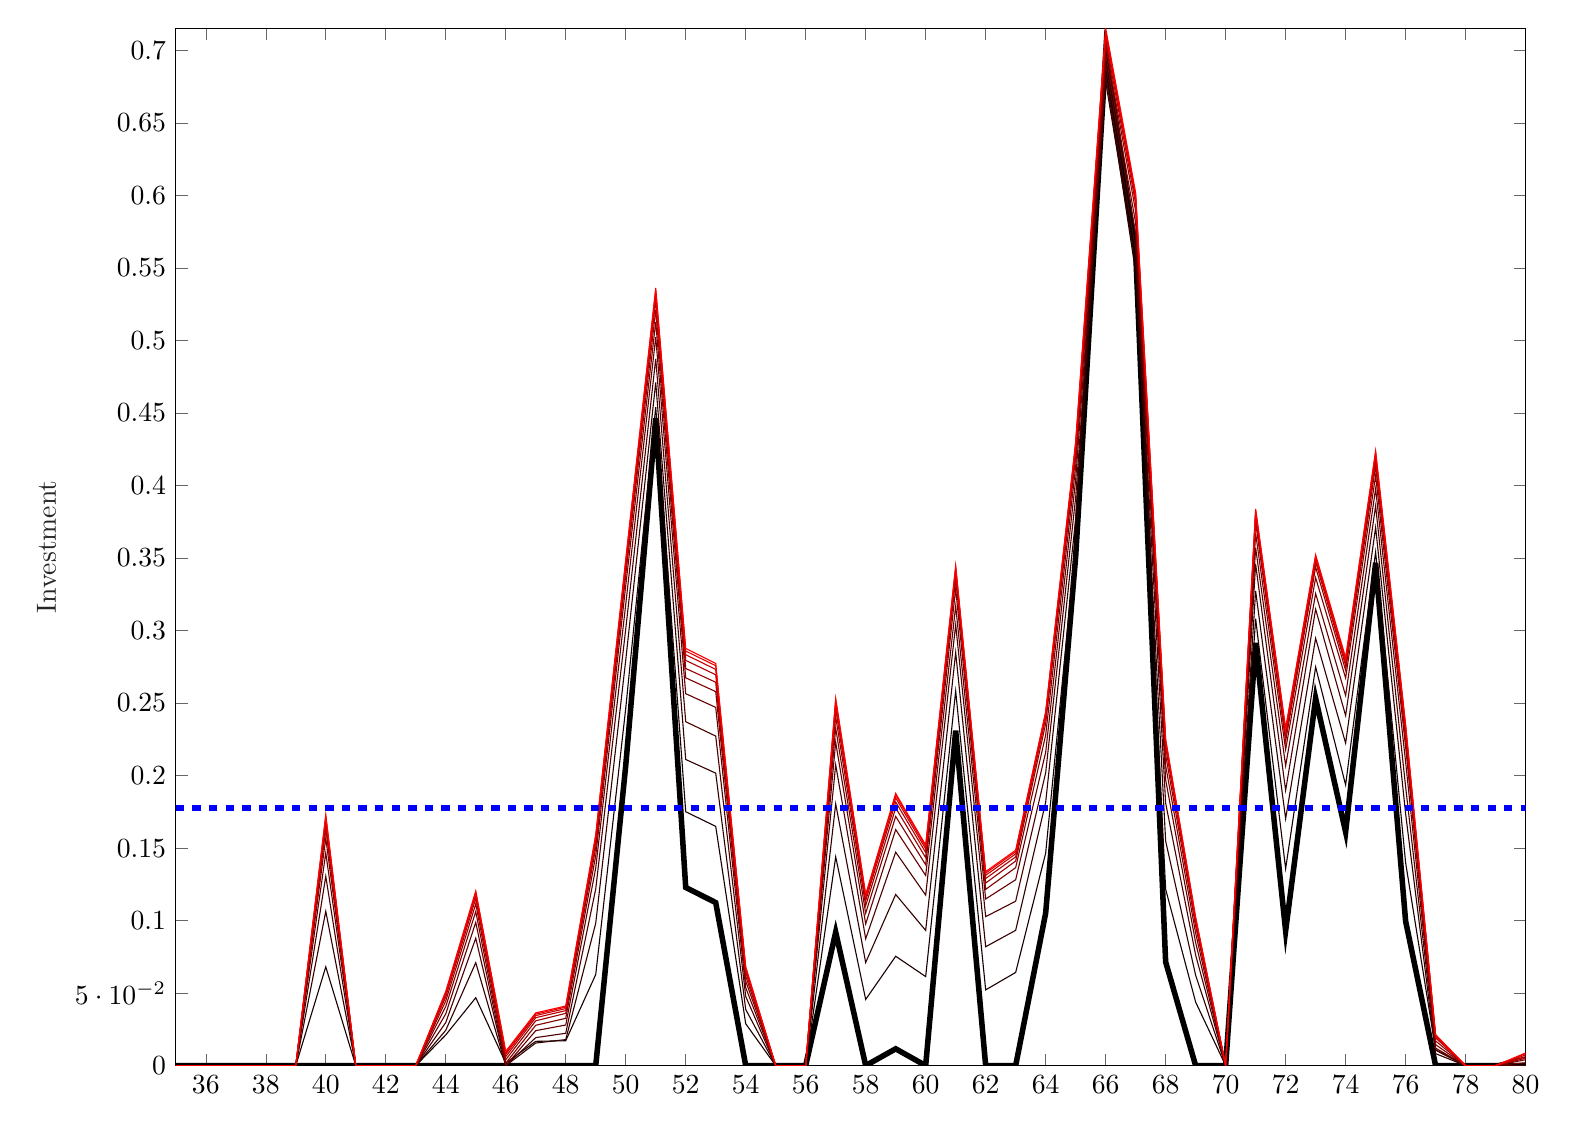
\begin{tikzpicture}

\begin{axis}[%
width=6.749in,
height=5.187in,
at={(1.132in,0.7in)},
scale only axis,
xmin=35,
xmax=80,
ymin=0,
ymax=0.715361118899045,
ylabel style={font=\color{white!15!black}},
ylabel={Investment},
axis background/.style={fill=white}
]
\addplot [color=black, line width=2.0pt, forget plot]
  table[row sep=crcr]{%
35	0\\
36	0\\
37	0\\
38	0\\
39	0\\
40	0\\
41	0\\
42	0\\
43	0\\
44	0\\
45	0\\
46	0\\
47	0\\
48	0\\
49	0\\
50	0.206912758260623\\
51	0.446325986384799\\
52	0.122858913259821\\
53	0.112422666773611\\
54	0\\
55	0\\
56	0\\
57	0.0920177891448049\\
58	0\\
59	0.011594070835933\\
60	0\\
61	0.230954610167834\\
62	0\\
63	0\\
64	0.105162150840503\\
65	0.351010667395535\\
66	0.697319916241752\\
67	0.561591796942152\\
68	0.0714783607376064\\
69	0\\
70	0\\
71	0.29145837619945\\
72	0.092956919383731\\
73	0.253298190701511\\
74	0.161126885973881\\
75	0.346750552117695\\
76	0.0996759714893127\\
77	0\\
78	0\\
79	0\\
80	0\\
};
\addplot [color=black!90!red, forget plot]
  table[row sep=crcr]{%
35	0\\
36	0\\
37	0\\
38	0\\
39	0\\
40	0.0681117903625863\\
41	0\\
42	0\\
43	0\\
44	0.0211613921163292\\
45	0.0468116052971943\\
46	0.00174778893469085\\
47	0.0167505358964546\\
48	0.0171504739568578\\
49	0.0628220730225133\\
50	0.246277837311223\\
51	0.454057133729556\\
52	0.175063423609477\\
53	0.164963941982203\\
54	0.0288731586179249\\
55	0\\
56	0\\
57	0.143934615686223\\
58	0.0456380019371685\\
59	0.0754148804910108\\
60	0.0613860656362135\\
61	0.258300586553547\\
62	0.0522360885943402\\
63	0.0642563148042232\\
64	0.146501697112415\\
65	0.359279202238604\\
66	0.683995715250124\\
67	0.547052793643154\\
68	0.121623973559258\\
69	0.0438107636106251\\
70	0\\
71	0.308193714081061\\
72	0.135786573358104\\
73	0.27486393567591\\
74	0.193560518623753\\
75	0.354145849432735\\
76	0.139943358247126\\
77	0.0109334954315852\\
78	0\\
79	0.00100154827092602\\
80	0.00600592689758072\\
};
\addplot [color=black!80!red, forget plot]
  table[row sep=crcr]{%
35	0\\
36	0\\
37	0\\
38	0\\
39	0\\
40	0.106415674835447\\
41	0\\
42	0\\
43	0\\
44	0.024357671220949\\
45	0.0709779331016356\\
46	0\\
47	0.0155765518773743\\
48	0.0179566611977335\\
49	0.0982137322709781\\
50	0.279523616110176\\
51	0.471032143738487\\
52	0.211104054377548\\
53	0.201690933048751\\
54	0.0387832717251009\\
55	0\\
56	0\\
57	0.180446972053508\\
58	0.0710951693201462\\
59	0.118020937927589\\
60	0.0932402412345885\\
61	0.284911045410003\\
62	0.0819903724304649\\
63	0.0932905783325557\\
64	0.181517486748944\\
65	0.376956529871418\\
66	0.678584457316284\\
67	0.553032382683017\\
68	0.154829196092543\\
69	0.0622915641080801\\
70	0\\
71	0.327287056516688\\
72	0.170291524851922\\
73	0.294658100368522\\
74	0.222369772600672\\
75	0.371162083772933\\
76	0.1736755781056\\
77	0.00827869683357418\\
78	0\\
79	0\\
80	0\\
};
\addplot [color=black!70!red, forget plot]
  table[row sep=crcr]{%
35	0\\
36	0\\
37	0\\
38	0\\
39	0\\
40	0.130567677969462\\
41	0\\
42	0\\
43	0\\
44	0.0297071418210097\\
45	0.0878822626507329\\
46	0\\
47	0.0193103489945729\\
48	0.0223000772109851\\
49	0.121794813254912\\
50	0.301037918300028\\
51	0.487392306532769\\
52	0.23713776855326\\
53	0.227245833447838\\
54	0.0477277973021204\\
55	0\\
56	0\\
57	0.207439916375051\\
58	0.0874617429940212\\
59	0.147187208463223\\
60	0.117586627719436\\
61	0.304019987424648\\
62	0.102726993219542\\
63	0.113372670178651\\
64	0.201917569569957\\
65	0.391758030661213\\
66	0.682796091913215\\
67	0.562759322317173\\
68	0.180991370691665\\
69	0.076224303094289\\
70	0\\
71	0.345782773683825\\
72	0.189793058582534\\
73	0.31473693305071\\
74	0.241368580534322\\
75	0.385924022227085\\
76	0.192348267056184\\
77	0.0105844125157071\\
78	0\\
79	0\\
80	0\\
};
\addplot [color=black!60!red, forget plot]
  table[row sep=crcr]{%
35	0\\
36	0\\
37	0\\
38	0\\
39	0\\
40	0.146671753310933\\
41	0\\
42	0\\
43	0\\
44	0.0357024924667959\\
45	0.0987760043408454\\
46	0\\
47	0.0241251911748879\\
48	0.027997243148399\\
49	0.136280111876889\\
50	0.318029016603176\\
51	0.502302022382199\\
52	0.256481362991278\\
53	0.247042304676943\\
54	0.0537616353671089\\
55	0\\
56	0\\
57	0.222964053904698\\
58	0.0976889943670942\\
59	0.16275053739878\\
60	0.131104163639335\\
61	0.316935160005611\\
62	0.114918495259294\\
63	0.128180461793758\\
64	0.216038840222609\\
65	0.403984570505078\\
66	0.690096041887973\\
67	0.573756188481209\\
68	0.19716914378205\\
69	0.0847648058718482\\
70	0\\
71	0.357090280730415\\
72	0.206774785429782\\
73	0.325510121945014\\
74	0.255194671105243\\
75	0.397766950819866\\
76	0.209347379324695\\
77	0.0120893172341192\\
78	0\\
79	0\\
80	0.00201275192076444\\
};
\addplot [color=black!50!red, forget plot]
  table[row sep=crcr]{%
35	0\\
36	0\\
37	0\\
38	0\\
39	0\\
40	0.156805282544082\\
41	0\\
42	0\\
43	0\\
44	0.0407708586422433\\
45	0.106188669069305\\
46	0.00171496688099482\\
47	0.0278143805307367\\
48	0.0326170948581634\\
49	0.144748863970502\\
50	0.330817710196351\\
51	0.512700381535334\\
52	0.267414160107469\\
53	0.2579036881991\\
54	0.0582922704132751\\
55	0\\
56	0\\
57	0.232637733832658\\
58	0.105078400597791\\
59	0.171803513239536\\
60	0.13852039136386\\
61	0.328809071735712\\
62	0.121540001705527\\
63	0.136513318014999\\
64	0.227867158290283\\
65	0.413034548798028\\
66	0.697014761232125\\
67	0.581135601864793\\
68	0.206875821453857\\
69	0.0913022657241946\\
70	0\\
71	0.366974267830061\\
72	0.217908514772061\\
73	0.336437647755389\\
74	0.267245179849641\\
75	0.406862168744479\\
76	0.219791063376011\\
77	0.0144770613395519\\
78	0\\
79	0\\
80	0.00405573043783769\\
};
\addplot [color=black!40!red, forget plot]
  table[row sep=crcr]{%
35	0\\
36	0\\
37	0\\
38	0\\
39	0\\
40	0.16313999990383\\
41	0\\
42	0\\
43	0\\
44	0.0446181696475938\\
45	0.111471169215879\\
46	0.00409999395808902\\
47	0.0309134592287361\\
48	0.0360351047074721\\
49	0.150194462656308\\
50	0.33813302237664\\
51	0.520963821800648\\
52	0.273874681479601\\
53	0.264375892426975\\
54	0.0617791778645535\\
55	0\\
56	0\\
57	0.240485313501495\\
58	0.110320102225508\\
59	0.17765600306589\\
60	0.14341492657476\\
61	0.335999332185346\\
62	0.125885365660744\\
63	0.141092910282964\\
64	0.23582332632736\\
65	0.419752322871557\\
66	0.703247801163574\\
67	0.589100759247454\\
68	0.214321281191051\\
69	0.0960710058380955\\
70	0\\
71	0.37452101378913\\
72	0.22366795095235\\
73	0.34368077712592\\
74	0.272605666126184\\
75	0.413541253511453\\
76	0.225125427404395\\
77	0.0170056142715214\\
78	0\\
79	0\\
80	0.00505602069957911\\
};
\addplot [color=black!30!red, forget plot]
  table[row sep=crcr]{%
35	0\\
36	0\\
37	0\\
38	0\\
39	0\\
40	0.167106633140723\\
41	0\\
42	0\\
43	0\\
44	0.0474068035601009\\
45	0.115222224235801\\
46	0.00621326584703019\\
47	0.0330521860924273\\
48	0.0379466803977728\\
49	0.153903751673674\\
50	0.342567131833056\\
51	0.527413519205792\\
52	0.279431096747759\\
53	0.269534512872381\\
54	0.064464213757504\\
55	0\\
56	0\\
57	0.245944125315474\\
58	0.113772459955472\\
59	0.181788270882988\\
60	0.146974091256365\\
61	0.339810732425141\\
62	0.129009586130059\\
63	0.143934130326027\\
64	0.239728818653802\\
65	0.424078831734667\\
66	0.70746191740563\\
67	0.594326956063375\\
68	0.219434715754488\\
69	0.0987954211360202\\
70	0\\
71	0.37860148373816\\
72	0.226806608296756\\
73	0.347323250675835\\
74	0.27588800771343\\
75	0.417586343632361\\
76	0.228727854403403\\
77	0.0190873318372542\\
78	0\\
79	0\\
80	0.00600729683528844\\
};
\addplot [color=black!20!red, forget plot]
  table[row sep=crcr]{%
35	0\\
36	0\\
37	0\\
38	0\\
39	0\\
40	0.169962364787538\\
41	0\\
42	0\\
43	0\\
44	0.0492572621046447\\
45	0.11769929439943\\
46	0.00786386236738789\\
47	0.0345066825826126\\
48	0.0393439735382426\\
49	0.156394485509749\\
50	0.345434255142012\\
51	0.531621196009331\\
52	0.283353478930727\\
53	0.273215401771478\\
54	0.0663232055037659\\
55	0\\
56	0\\
57	0.249486570269065\\
58	0.11585459285615\\
59	0.184614121543195\\
60	0.149398525888008\\
61	0.342053294515015\\
62	0.131198579663252\\
63	0.146012816133238\\
64	0.241957817213452\\
65	0.426977147533611\\
66	0.711118527392388\\
67	0.597661867808498\\
68	0.222636359640798\\
69	0.100601499795512\\
70	0\\
71	0.380954565942905\\
72	0.229339958317151\\
73	0.349360797519566\\
74	0.277964845214992\\
75	0.420599050758286\\
76	0.231864534311277\\
77	0.020268730525538\\
78	0\\
79	0\\
80	0.00727348087991375\\
};
\addplot [color=black!10!red, forget plot]
  table[row sep=crcr]{%
35	0\\
36	0\\
37	0\\
38	0\\
39	0\\
40	0.171754039392575\\
41	0\\
42	0\\
43	0\\
44	0.0503797527646557\\
45	0.119467524317999\\
46	0.0090473167315479\\
47	0.0355124377090945\\
48	0.0403539542536082\\
49	0.158132511646645\\
50	0.347545973602497\\
51	0.53451812252946\\
52	0.285885742581521\\
53	0.275770557553196\\
54	0.0674876738314587\\
55	0\\
56	0\\
57	0.251799535841536\\
58	0.117208647256008\\
59	0.186484128855344\\
60	0.151026359580838\\
61	0.34356877009719\\
62	0.132733112855797\\
63	0.147511553702\\
64	0.243213266029993\\
65	0.42907897059573\\
66	0.713515957044485\\
67	0.600039380584835\\
68	0.224262732580199\\
69	0.101645463698508\\
70	0\\
71	0.38262094674385\\
72	0.231327629635072\\
73	0.350979415322803\\
74	0.279884412095189\\
75	0.422627242444269\\
76	0.233977738992102\\
77	0.0209295810047918\\
78	0\\
79	0\\
80	0.00821650206871016\\
};
\addplot [color=red, forget plot]
  table[row sep=crcr]{%
35	0\\
36	0\\
37	0\\
38	0\\
39	0\\
40	0.172857147597689\\
41	0\\
42	0\\
43	0\\
44	0.0511981633671694\\
45	0.120414815350031\\
46	0.00988874687401652\\
47	0.0363732749912582\\
48	0.0410795750627948\\
49	0.159266049313152\\
50	0.349092388353274\\
51	0.536199621222013\\
52	0.287665730745454\\
53	0.277353792515928\\
54	0.0682028962300156\\
55	0\\
56	0\\
57	0.253309749789706\\
58	0.117966836307206\\
59	0.187725128407274\\
60	0.15213452648711\\
61	0.344730219048969\\
62	0.13376723076841\\
63	0.148535751958996\\
64	0.243970559582037\\
65	0.430317645662782\\
66	0.715361118899045\\
67	0.601935680318696\\
68	0.225150094156996\\
69	0.102312025334615\\
70	0\\
71	0.383907543893641\\
72	0.232648362342682\\
73	0.352198304957331\\
74	0.281399568372125\\
75	0.423967091714583\\
76	0.235363236901556\\
77	0.0213938703037113\\
78	0\\
79	0\\
80	0.00873377852301238\\
};
\addplot [color=blue, dashed, line width=2.0pt, forget plot]
  table[row sep=crcr]
  \end{center}

\end{frame}


\end{document}
